%% LyX 2.2.0 created this file.  For more info, see http://www.lyx.org/.
%% Do not edit unless you really know what you are doing.
\documentclass[11pt,english,american,draftfoot]{ulb_thesis}
\usepackage[T1]{fontenc}
\usepackage[latin9]{inputenc}
\usepackage{float}
\usepackage{url}
\usepackage{pdfpages}
\usepackage{slashed}
\usepackage{amsmath}
\usepackage{amssymb}
\usepackage{stmaryrd}
\usepackage{makeidx}
\makeindex

\makeatletter

%%%%%%%%%%%%%%%%%%%%%%%%%%%%%% LyX specific LaTeX commands.
%% Because html converters don't know tabularnewline
\providecommand{\tabularnewline}{\\}
%% A simple dot to overcome graphicx limitations
\newcommand{\lyxdot}{.}

\floatstyle{ruled}
\newfloat{algorithm}{tbp}{loa}[chapter]
\providecommand{\algorithmname}{Algorithm}
\floatname{algorithm}{\protect\algorithmname}

%%%%%%%%%%%%%%%%%%%%%%%%%%%%%% Textclass specific LaTeX commands.
 \input{ulb_ntheorem.std}
\newenvironment{lyxlist}[1]
{\begin{list}{}
{\settowidth{\labelwidth}{#1}
 \setlength{\leftmargin}{\labelwidth}
 \addtolength{\leftmargin}{\labelsep}
 \renewcommand{\makelabel}[1]{##1\hfil}}}
{\end{list}}

%%%%%%%%%%%%%%%%%%%%%%%%%%%%%% User specified LaTeX commands.
\usepackage{tikz, pgf, pgfplots}
\usetikzlibrary{automata,graphs,positioning}
\usetikzlibrary{arrows,backgrounds,plotmarks}
\pgfplotsset{width=7cm,compat=newest}
\pgfplotsset{plot coordinates/math parser=false}

\@ifundefined{showcaptionsetup}{}{%
 \PassOptionsToPackage{caption=false}{subfig}}
\usepackage{subfig}
\makeatother

\usepackage{babel}
\addto\captionsenglish{\renewcommand{\algorithmname}{Algorithm}}

\begin{document}
\includepdf{PageDeGarde}
\begin{dedication}
To my parents.
\end{dedication}
\begin{acknowledgments}
Thank you, my advisor!
\end{acknowledgments}
\vspace*{4cm}

\emph{``A great citation here}''

\begin{flushright}
X
\par\end{flushright}
\begin{abstract}
abstract of the thesis
\end{abstract}
\tableofcontents{}

\listoffigures

\listoftables

\mainmatter

\selectlanguage{english}%

\chapter{Introduction}


\section{Problem}

citation example \cite{book-full}


\section{Objective}

index example\index{example@\selectlanguage{american}%
example\selectlanguage{american}%
}


\section{Outline}

blabla


\section{Contributions}

blabla


\section{Publications}

blabla


\section{Notations}

blabla\selectlanguage{american}%



\chapter{Information Extraction}

In this chapter, I give a generic introduction to Information Extraction.
This Chapter is a re-elaboration of \cite{Sarawagi:2008:IE:1498844.1498845}.
Please refer to the original source for a more comprehensive and detailed
overview. The figures and examples appearing in this Chapter are mine.

\section{Definition}

Information Extraction (IE) is the discipline that addresses the task
of extracting structured information from unstructured sources automatically.
Sources usually take the form of text documents. The most explored
aspect of IE is the extraction of \emph{named entities.} Another main
topic, that has become object of research only in recent years, is
the extraction of \emph{relationships} between entities. IE is a field
with contributions from many different communities: Machine Learning,
Information Retrieval, Database, Web, Document Analysis. The interest
towards it is motivated by the constantly increasing amount of data
that is generated by our society. Manual analysis has become infeasible.
IE promises to bring value to many application domains, most notably
the enterprise world and the Web.

\medskip{}

There are two prominent approaches to IE: 
\begin{description}
\item [{\emph{rule-based}}] which define a set of rules that the output
has to respect. The rules can be manually coded or learnt from examples;
\item [{\emph{statistical}}] which seek to identify a decomposition of
unstructured text and to label its components.
\end{description}

\section{Example Applications}

\paragraph{News Tracking}

The activity of tracking events in news articles. It can result in
a lot of useful services, like automatic creation of multimedia news,
linking articles to information pages on the entities found, etc.

\paragraph{Data Cleaning}

Extracting structured forms from flat data strings (containing, e.g.,
addresses). It allows more effective deduplication of information,
among the other things.

\paragraph{Citation Databases}

Articles, conference sites, individual research sites and similar
are explored to obain formatted citations of publications, later stored
in publicly accessible databases. They are capable to forward references
and may provide aggregate statistics and scoring information. See,
for instance, Google Scholar (\url{https://scholar.google.com/}).

\paragraph{Relationship Web Search}

Relationship extraction would be a very useful feature to integrate
into web search engines, as the keyword search that they offer at
present time is only good for entity identification.

\section{Issues}

The main issues that have to be dealt with when performing IE can
be divided in two categories: \emph{accuracy} and \emph{running time}.

\subsection{Accuracy}

We measure the accuracy of an IE task with two quantities:
\begin{itemize}
\item \emph{precision}: the percentage of correctly extracted entities among
the extracted entities;
\item \emph{recall}: the percentage of entities extracted among all the
existing entities in the input source.
\end{itemize}
The main difficulties to achieving a good level of accuracy are:
\begin{itemize}
\item the availability of a great set of clues that might be very different
in nature (e. g. orghographic properties, part of speech, typical
words, etc.) and that might be difficult to combine;
\item the difficulty of finding out missed extractions;
\item the fact that with the advancement of research the extracted data
structures keep increasing in complexity (for instance it is becoming
more difficult to identify the boundaries of an entity in a text).
\end{itemize}
While it is possible to reach a very good level of accuracy for entity
extraction ($90\%$), relationship extraction is still quite unreliable
($50-70\%$ accuracy), mainly due to its intrinsic complexity.

\subsection{Running Time}

In its initial phase IE was interesting only to research communities.
Nowadays companies, because of the enormous amount of data they need
to process on a regular basis, are concerned with IE too, and \emph{scalability}
has become a central issue, while many IE systems don't address the
problem of efficiently carrying out extraction tasks with sufficient
attention. Efficiency is influenced most notably by the efficiency
of the following tasks:
\begin{itemize}
\item filtering documents in order to actually examine only the ones that
have good chances to contain the desired information;
\item focusing on the parts of a document that contain relevant information;
\item processing steps, like database querying, that are typically very
expensive and that might have to be performed on the selected pieces
of input.
\end{itemize}
Recently many solutions have been proposed to target the scalability
issue; one of these is SystemT.

\section{Entity Extraction\label{sec:Entity-Extraction}}

Named entities are elements of interest in a text. Example of entities
are person names, street addresses, institutions, countries, and so
on. In this section and in the next one, I assume that the output
of an extraction task is a series of labels inserted into an input
text document (that becomes \emph{annotated}), although there are
other possible output formats.

\subsection{Rule-based Methods}

Rule-based methods employ sets of predicates that are ``fired''
independently. When a portion of input text satisfies a predicate,
the predicate's associated action is executed. A predicate can be
represented in the following generic form:

\begin{equation}
\textrm{"Contextual Pattern}\longrightarrow\textrm{Action"}
\end{equation}
Contextual patterns are a way to identify entitities by exploiting
their properties or the context in which they are usually met. The
most common formalism used to express them is that of \emph{regular
expressions} over tokens of the input. Actions mark the entities that
have been identified, and might consist in storing them in a database
or adding delimiters directly in the text.

Most systems in this category present a \emph{cascaded structure}:
an input document goes through a series of processing phases, and
the output of a phase is the input of the next one. A famous example
is that of \emph{cascading grammars}: formal grammars are evaluated
in sequence on the input.

As I said, a contextual pattern seeks for (groups of) tokens that
have certain features. In the case of entity extraction, features
can be classified in the following categories:
\begin{itemize}
\item string representation;
\item orthography (e.g. small case, mixed case, number, etc.);
\item part of speech;
\item list of dictionaries they're contained into;
\item annotation obtained in previous phases.
\end{itemize}
Rules can be hand-coded by experts or learned through learning algorithms.
In the second case the goal is to cover each of the entities of interest
in the training set with at least one rule. The obtained rules should
have good recall and precision on new input. Moreover, when learning
a set of rules, we would like to achieve a good level of \emph{generalizability},
that is: we would like to find the minimum set of rules accounting
for the maximum portion of training data, with high precision. There
are two main strategies for rule learning: \emph{bottom-up} (start
from very specific rules and make them more and more general) and
\emph{top-down} (start with rules covering all existing instances,
then specialize them).

\subsubsection{Example Rules}

For the examples I use an idealized syntax, as in \cite{Sarawagi:2008:IE:1498844.1498845}.
\begin{example}
Consider the task of identifying all mentions ISO standards in a text.
A rule for this purpose could be:

\begin{multline}
\left(\left\{ \textrm{String}=\textrm{"ISO"}\right\} \left\{ \textrm{String}=\textrm{"/IEC"}\right\} \left\{ \textrm{?}\right\} \left\{ \textrm{String}=\textrm{"/ASTM"}\right\} \left\{ \textrm{?}\right\} \right.\\
\left.\left\{ \textrm{Orthography type}=\textrm{number}\right\} \left\{ \left\{ \textrm{String}=\textrm{":"}\right\} \left\{ \textrm{Orthography type}=\textrm{number}\right\} \right\} \left\{ \textrm{?}\right\} \right)\\
\longrightarrow\textrm{ISO Standards}
\end{multline}
\end{example}

\begin{example}
Multiple entities can be matched at once. Imagine we need to find
mentions of (simple) street addresses in a text consisting of a street
name and a street number. A rule that matches the name and number
separatedly could be:

\begin{multline}
\left(\left\{ \textrm{Orthography type}=\textrm{mixed case word}\right\} \left\{ \textrm{*}\right\} \right)\textrm{: Name}\left(\left\{ \textrm{String}=\textrm{","}\right\} \right)\\
\left(\left\{ \textrm{Orthography type}=\textrm{number}\right\} \right)\textrm{: Number}\\
\longrightarrow\textrm{Street Name}=:\textrm{Name, }\textrm{Street Number}=:\textrm{Number}
\end{multline}
\end{example}


\subsection{Statistical Methods}

Statistical methods aim to decompose the source, assigning a label
to each element in the decomposition. We distinguish between three
types of statistical models:
\begin{itemize}
\item \emph{Token-level models}: they assign a label to each token of the
source. Since entities are usually comprised of multiple adjacent
tokens, the tags used are of the forms ``entity\_begin'', ``entity\_continue'',
``entity\_end'';
\item \emph{Segment-level models}: they try to find the best segmentation
of the source text;
\item \emph{Grammar-based models: }they use formal grammars, outputting
parse trees. All the valid parses are considered for an input document,
assigning a score to each. The parse with the highest score is retained.
\end{itemize}
I now give a brief description of Token-level Models and Segment-level
Models.

\subsubsection{Token-Level Models\label{subsec:Token-Level-Models}}

\paragraph{Features}

The clues that these models exploit are of the form 
\begin{equation}
f:\left(\mathbf{x},y,i\right)\longmapsto\mathbb{R}
\end{equation}
where $\mathbf{x}$ is a sequence of tokens, $i$ is a position in
$\mathbf{x}$ and $y$ is a candidate label for the token at $i$.
We distinguish between these types of features:
\begin{itemize}
\item \emph{word features};
\item \emph{orthographic features;}
\item \emph{dictionary lookup features.}
\end{itemize}
\begin{figure}
Yesterday I watched a movie called ``The Matrix''

\begin{tabular}{|c|c|c|c|c|c|c|c|c|c|c|}
\hline 
i & 1 & 2 & 3 & 4 & 5 & 6 & 7 & 8 & 9 & 10\tabularnewline
\hline 
\hline 
x & Yesterday & I & watched & a & movie & called & `` & The & Matrix & ``\tabularnewline
\hline 
y & $y_{1}$ & $y_{2}$ & $y_{3}$ & $y_{4}$ & $y_{5}$ & $y_{6}$ & $y_{7}$ & $y_{8}$ & $y_{9}$ & $y_{10}$\tabularnewline
\hline 
\end{tabular}

\caption{\label{fig:tokenization}Decomposition of a sentence into a sequence
of tokens.}
\end{figure}

\begin{example}
Consider the sentence shown in Figure \ref{fig:tokenization} and
its corresponding decomposition. An example of word feature at position
5 is

\[
f_{1}\left(y,\mathbf{x},i\right)=\left\llbracket x_{i}\textrm{ equals "Matrix"}\right\rrbracket \cdot\left\llbracket y=\textrm{Movie}\right\rrbracket 
\]
where $\left\llbracket P\right\rrbracket =1$ if predicate $P$ is
true, and 0 otherwise. An orthographic feature might be

\[
f_{2}\left(y,\mathbf{x},i\right)=\left\llbracket x_{i}x_{i+1}\textrm{ matches INITIAL\_QUOTE CapsWord}\right\rrbracket \cdot\left\llbracket y=\textrm{Movie}\right\rrbracket .
\]

Finally, an example of dictionary lookup feature is

\[
f_{3}\left(y,\mathbf{x},i\right)=\left\llbracket x_{i}\textrm{ in Movie\_dictionary}\right\rrbracket \cdot\left\llbracket y=\textrm{Movie}\right\rrbracket .
\]
\end{example}


\paragraph{Models for Labeling Tokens}

The best models are the ones that take into account dependencies between
tokens, among which we may find:
\begin{itemize}
\item \emph{ordered classifiers};
\item \emph{Hidden Markov models;}
\item \emph{Maximum Entropy Taggers;}
\item \emph{Conditional Markov Models;}
\item \emph{Conditional Random Fields }(the state of the art).
\end{itemize}

\subsubsection{Segment-Level Models}

\paragraph{Features}

In these models the label for a segment depends on the properties
of its tokens and on the previous segment. We can describe a segment
$s_{j}$ as:
\begin{equation}
s_{j}=\left(y_{i},l_{j},u_{j}\right)\label{eq:segment}
\end{equation}
where $y_{i}$ is the proposed label for $s_{j}$ and $l_{j},u_{j}$
are the start and end positions of $s_{j}$. Therefore, a feature
is of the form:
\begin{equation}
f\left(y_{i},y_{i-1},\mathbf{x},l_{j},u_{j}\right)
\end{equation}
where $\mathbf{x}$ is the input sequence of tokens, $y_{i-1}$ is
the proposed label for the previous segment and the other symbols
are defined as for Equation \ref{eq:segment}. Besides token-level
features (see Subsection \ref{subsec:Token-Level-Models}), we can
exploit the following feature types:
\begin{itemize}
\item \emph{Similarity to an entity in a database;}
\item \emph{Length of the segment.}
\end{itemize}
\begin{figure}
``The Matrix'' by The Wachowski Brothers

\begin{tabular}{|c|c|c|c|}
\hline 
i & %
\begin{tabular}{cccc}
1 & 2 & 3 & 4\tabularnewline
\end{tabular} & 5 & %
\begin{tabular}{ccc}
6 & 7 & 8\tabularnewline
\end{tabular}\tabularnewline
\hline 
\hline 
x & ``The Matrix'' & by & The Wachowski Brothers\tabularnewline
\hline 
$\left(l_{j},u_{j},y_{i}\right)$ & $1,4,M$ & $5,5,O$ & $6,8,D$\tabularnewline
\hline 
\end{tabular}

\caption{\label{fig:segmentation2}Segmentation of a sentence.}
\end{figure}

\begin{example}
Consider the sentence in Figure \ref{fig:segmentation2} and its corresponding
segmentation, which identifies a movie and a director. A basic feature
similarity feature for the director could be:

\[
f\left(y_{i},y_{i-1},\mathbf{x},6,8\right)=\left\llbracket x_{6}x_{7}x_{8}\textrm{ appears in a list of movie directors}\right\rrbracket \cdot\left\llbracket y_{i}=\textrm{Director}\right\rrbracket .
\]

A more realistic feature would make use of some similarity function,
rather than requiring an extact match. An example of length feature
is

\[
f\left(y_{i},y_{i-1},\mathbf{x},l,u\right)=\left\llbracket u-l=3\right\rrbracket \cdot\left\llbracket y_{i}=\textrm{Director}\right\rrbracket .
\]

\medskip{}
\end{example}

There exist also global segmentation models, that try to find the
best segmentation of a token sequence by maximizing a target function.

\section{Relationship Extraction}

When exctracting relationships between entities, we might face three
types of specific tasks:
\begin{enumerate}
\item given a pair of entities, find the relationship between them;
\item given an entity $e$ and a relationship $r$, find all the other entities
$e'$ such that $\left(e,e'\right)\in r$;
\item given a big and open-ended input and a relationship $r$ find all
pairs of entities $e',e''$ such that $\left(e',e''\right)\in r$.
\end{enumerate}

\subsection{Predicting the Relationship between an a Pair of Entities}

For the first task, we can exploit the following resources:
\begin{itemize}
\item \emph{surface tokens}: tokens that are usually placed between entities.
They are strong clues;
\item \emph{part of speech tags }(the most important being verbs);
\item \emph{syntactic parse tree}: allows grouping words in phrase types,
e.g. noun phrases, propositional phrases, and so on;
\item \emph{dependency graph}: it is a less expensive structure to compute
than the parse tree and it links a word to those that depend on it.
\end{itemize}
The main methods available to carry out the task are:
\begin{itemize}
\item \emph{Feature-based methods}, that simply transform the clues mentioned
above for usage by conventional classifier models;
\item \emph{Kernel-based methods}, that use kernel functions to encode the
similarity between two graphs;
\item \emph{Rule-based methods}, creating rules over structures around pairs
of entities.
\end{itemize}
The second task is a special case of the third, and won't be treated
here.

\subsection{Finding All Possible Entity Pairs Belonging to a Relationship}

The third task can be met especially when dealing with the Web. Usually
we can exploit the following resources to fulfill it:
\begin{itemize}
\item the \emph{types of arguments} of $r$ (that might need specific recognition
patterns);
\item a \emph{seed database} of pairs of entities belonging to $r$;
\item \emph{manually coded patterns}.
\end{itemize}
The generic procedure that is used in this case can be described with
these steps:
\begin{enumerate}
\item Use the seed database to learn the relevant extraction patterns;
\item Use the obtained patterns to define candidate triples of the form
$\left(e',e'',r\right)$;
\item Retain a subset of the candidate triples, using a statistical test.
\end{enumerate}
There exist also rule-based methods for the task. 

\chapter{SystemT and AQL}

In this chapter, I give a description of \emph{SystemT} and its extraction
rule language \emph{AQL} (Annotation Query Language), and of a new
way of evaluating AQL queries, that uses a formalism derived from
\emph{Finite State Automata}. This chapter is a re-elaboration from
\cite{4497502,Krishnamurthy:2009:SSD:1519103.1519105,Fagin:2015:DSF:2772377.2699442}.
In particular, the mathematical statements from \ref{first-stat}
to \ref{.last-stat} are taken or adapted from \cite{Fagin:2015:DSF:2772377.2699442},
except for Remarks \ref{first-rem} to \ref{last-rem}, that come
from \cite{4497502}. Please refer to the original sources for more
details on the topic. The figures and examples appearing in this chapter
are mine, except when I explicitly state otherwise.

\section{SystemT}

As I mentioned in the previous chapter, scalability is now a main
concern in IE. Companies rely on IE for many tasks; a prominent example
is \emph{Business Intelligence}. Unfortunately, many systems developed
in the past don't address this issue correctly. Traditionally, most
rule-based system rely on cascading grammars: formal grammars are
executed in sequence on the input, each grammar representing a stage
that takes as input the ouput of the previous one. Rules in such grammars
are matched using regular expressions: if a part of the input text
satisfies the regular expression associated with a rule, that rule
is activated (i.e. ``fires'') and the corresponding action is executed.
Evaluating a grammar on a document tends to be costly, because simply
evaluating a single rule might require scanning the whole document.
On large datasets, the running time becomes enormous. What's more,
these kind of systems are not able to fulfill the expressivity requirements
of the complex extraction tasks.

SystemT was developed at IBM to address these issues. This system
is based on a new approach to extraction rules: the \emph{algebraic
approach}. Here, data manipulations are viewed as operations in a
(relational) algebra. Extraction tasks are defined using \emph{annotators}
(see Section \ref{sec:Entity-Extraction}) whose rules are viewed
as \emph{queries} on input documents, that act as virtual databases.
Complex annotators are obtained by combining simple ones by means
of \emph{relational operators}. By doing so, all the optimization
techniques used in regular databases become available, but new techniques
are possible too, due to the characteristics of text documents. Another
advantage of SystemT is that it is capable to handle \emph{overlapping
rule matchings}, due to rulels being fired independently, which are
difficult to resolve in cascading grammars, where they tipically require
disambiguation policies that only partially solve the problem.

I now give an overview of SystemT's high-level structure. Then, I
talk about its data model, execution model and algebra. For more information
on SystemT and AQL, please refer to \cite{4497502,Krishnamurthy:2009:SSD:1519103.1519105}.

\subsection{Architecture}

These are the main components of SystemT:
\begin{description}
\item [{Development~Environment:}] allows constructing annotators for
extraction tasks. Rules are expressed in AQL, and compiled into an
algebra. It supports an iterative development process.
\item [{Optimizer:}] seeks for the best query plan for an extraction task,
evaluating the most convenient optimization techniques in a cost-based
manner.
\item [{Runtime~Environment:}] given a query plan, it instantiates the
physical operators corresponding to the logical ones in the plan,
then it proceeds evaluating it on input documents.
\end{description}
Once the development of an annotator is complete, it is \emph{published}
to the optimizer and runtime. After optimization, the runtime evaluates
it on a continuous stream of documents.

\subsection{Data Model\label{subsec:Data-Model}}

SystemT uses an \emph{object-relational} data model for annotations
on a text document, that allows applying logical operators over it.
Operators can be composed. There is an important assumption to mention
before continuing: an extraction task over a set of documents is performed
on one document at a time. This means that any relationships between
entities in different documents are disregarded. This assumption is
crucial to some optimization techniques that SystemT uses. While there
exist tasks where considering these relationships would be useful
(think of the Web), still a large number of relevant tasks can be
carried out this way. In the following, I report the definitions of
the basic data types in the data model of SystemT.

\medskip{}

I consider a finite alphabet $\Sigma$ of symbols (characters). $\Sigma^{*}$
denotes the set of all strings of finite length over $\Sigma$. A
document is modeled as one such string. 
\begin{definition}
\label{first-stat}A document is a string $\mathbf{s}\in\Sigma^{*}$.
\end{definition}

\noindent The most basic data type is the \emph{span}.
\begin{definition}
Given a string $\mathbf{s}=\sigma_{1}...\sigma_{n}$ where $\forall i$,
$\sigma_{i}\in\Sigma$, with length$\left|\mathbf{s}\right|=n$ and
whose characters are indexed in the natural way, a span is a substring
$\left[i,j\right\rangle $, where $i$, $j$ are indices of $s$ satisfying
$1\leq i\leq j\leq n+1$. A span of $\mathbf{s}$ is also denoted
as $\mathbf{s}_{\left[i,j\right\rangle }$.
\end{definition}

\noindent Spans can be aggregated in \emph{tuples}, which are finite
sequences of spans\emph{. }Let us denote the set of all possible spans
of a string $\mathbf{s}$ by $\textrm{Spans}\left(\mathbf{s}\right)$
and by $\textrm{SVars}$ an infinite set of span variables, which
can be assigned spans. A $\left(V,\mathbf{s}\right)-\textrm{tuple}$
is defined as follows:
\begin{definition}
Given a set $V\subseteq\textrm{SVars}$, $V$ being finite, and a
string $\mathbf{s}\in\sum^{*}$, a $\left(V,\mathbf{s}\right)-\textrm{tuple}$
is a mapping $\mu:V\longmapsto\textrm{Spans}\left(\mathbf{s}\right)$.
When $V$ is clear from the context, we might call $\mu$ simply a
$\mathbf{s}-\textrm{tuple}$.
\end{definition}

\noindent A set of tuples is called a \emph{relation. }Here, we focus
on \emph{span relations}, which are formally defined as $\left(V,\mathbf{s}\right)-\textrm{relations}$.
\begin{definition}
\label{span-relation}A $\left(V,\mathbf{s}\right)-\textrm{relation}$
is a set of $\left(V,\mathbf{s}\right)-\textrm{tuples}$. As before,
we can speak of $\mathbf{s}-\textrm{relation}$ when $V$ is clear.
\end{definition}

\noindent Each operator in the algebra of SystemT takes one or more
span relations as input and outputs a single span relation.

\subsection{Execution Model\label{subsec:Execution-Model}}

A single document is conceived as a \emph{local annotation database},
to which annotators are applied in order to build \emph{views}. In
general, a local database fits into main memory. Local databases are
contained in a \emph{global annotation database}. The runtime of SystemT
takes a global database and it annotates its local databases. The
procedure is described by Algorithm \ref{alg:Annotating-all-local}.

\begin{algorithm}
$E\longleftarrow\left\{ \textrm{algebra expression}\right\} $

for localDB in globalDB do

begin
\begin{enumerate}
\item $\left\{ \textrm{Read localDB into main memory}\right\} $
\item $R\longleftarrow E\left(\textrm{localDB}\right)$
\item $\left\{ \textrm{Add \ensuremath{R} to localDB}\right\} $
\item $\left\{ \textrm{Write modified localDB to disk}\right\} $
\end{enumerate}
\caption{\label{alg:Annotating-all-local}Annotating all local databases in
a global database (taken from \cite{4497502}).}

\end{algorithm}


\subsection{Algebra of Operators \label{subsec:Algebra-of-Operators}}

The operators of SystemT's algebra can be classified in three groups:
\begin{itemize}
\item \emph{relational operators;}
\item \emph{span extraction operators;}
\item \emph{span aggregation operators.}
\end{itemize}
In addition, there exist some \emph{span selection predicates} that
are used for span selection.

\subsubsection{Relational Operators}

Relational operators are the usual operators of relational algebra
that appear in classical database query plans. Important examples
are:
\begin{itemize}
\item \emph{selection} ($\sigma$);
\item \emph{projection }($\pi$);
\item \emph{Cartesian product }($\times$);
\item Join ($\bowtie$);
\item \emph{Union} ($\cup$);
\item \emph{Intersection} ($\cap$).
\end{itemize}

\subsubsection*{Span Extraction Operators}

Loosely speaking, span extraction operators take a pattern and a document
as input and output a maximal set of spans that match that pattern.
There are two main span extraction operators:
\begin{lyxlist}{00.00.0000}
\item [{\emph{standard~regular~expression~matcher~($\varepsilon_{re}$)}:}] this
operator takes a regular expression $r$ as input and it identifies
all non-overlapping matchings of $r$ in the current document, from
left to right.
\item [{\emph{dictionary~matcher~($\varepsilon_{d}$)}:}] this operator
outputs all the spans that match some entry in a given dictionary.
\end{lyxlist}
Although the dictionary matcher might seem useless since there is
a regular expression matcher, it has some advantages over it, as the
fact that it can find overlapping matchings or that it enforces the
semantics of word boundaries.

\subsubsection*{Span Aggregation Operators}

Span aggregation operators are used to aggregate spans in a meaningful
way. They are of two types:
\begin{itemize}
\item \emph{Consolidation}: they are used to coalesce overlapping spans
that were matched using patterns for the same concept. They are: 

\begin{lyxlist}{00.00.0000}
\item [{\emph{containment~consolidation~($\varOmega_{c}$)}:}] it discards
a span if it is fully contained into another one.
\item [{\emph{overlap~consolidation~($\varOmega_{o}$)}:}] it merges
spans that overlap repeatedly.
\end{lyxlist}
\item \emph{Block ($\beta$)}: it matches a series of spans, each at a distance
from its neighbor span(s) that is not superior to a threshold. It
is thought to identify regularity. It is tuned by two parameters:
a \emph{distance constraint} to control regularity and a \emph{count
constraint }that establishes the minimum number of spans in a block.
\end{itemize}

\subsubsection{Span Selection Predicates}

\noindent Consider two spans $s_{1},s_{2}$. The main span predicates
that may be used for selection are the following:
\begin{lyxlist}{00.00.0000}
\item [{$s_{1}\preceq_{d}s_{2}$}] \noindent when $s_{1},s_{2}$ do not
overlap, $s_{1}$ precedes $s_{2}$ and there are less than $d$ characters
between them;
\item [{$s_{1}\simeq s_{2}$}] when the two spans overlap;
\item [{$s_{1}\subset s_{2}$}] when $s_{1}$ is strictly contained in
$s_{2}$;
\item [{$s_{1}\subseteq s_{2}$}] when $s_{1}$ is contained in or equals
$s_{2}$;
\item [{$s_{1}=s_{2}$}] when $s_{1}$ equals $s_{2}$.
\end{lyxlist}
\begin{figure}
{\tiny{}``Yesterday I }\textbf{\tiny{}watched 'Annie Hall'}{\tiny{}.
It is about the relationship between a TV writer and his girlfriend,
who wants to become an actress. I really }\textbf{\tiny{}loved this
movie}{\tiny{}. Although the }\textbf{\tiny{}acting wasn't very good
}{\tiny{}sometimes, the }\textbf{\tiny{}dialogues were smart}{\tiny{}.
I'd recommend it to anyone.''}{\tiny \par}

\centering

\subfloat[\label{fig:high-level}High-level structure.]{\tikz[level distance=2cm]  	\node[rectangle, draw, align=center] {ReviewInstance \\ Aggregator}  		child { node[rectangle, draw, align=center] {ReviewPart \\ Extractor}  			edge from parent [<-] node[right=1.6cm, pos=1.5, draw=none, font=\tiny, align=left] {"watched 'Annie Hall'" \\ "loved this movie" \\ "acting wasn't very good" \\ "dialogues were smart"} 			edge from parent [<-] node[right=1.6cm, pos=-0.7, draw=none, font=\tiny, align=left] {"\textbf{watched 'Annie Hall'}. \\ It is about... \textbf{loved this} \\ \textbf{movie}. Altough the \textbf{acting} \\ \textbf{wasn't very good}... \\ \textbf{dialogues were smart}"}  		};

}

\subfloat[\label{fig:tree}Operator tree.]{\tikz [level distance=1.6cm, level 3/.style={sibling distance=6em}, level 4/.style={sibling distance=2em}] 	\node {$\varOmega_{c}$} 			child { node {$\beta$} 				child { node {$\cup$} 					child { node {$\bowtie_{\preceq_{10}}$} 						child { node {$\varepsilon_{d}$} edge from parent [<-] node[left,draw=none, font=\tiny] {Action} } 						child { node {$\varepsilon_{re}$} edge from parent [<-] node[right,draw=none, font=\tiny] {Title} } 						edge from parent [<-] node[left, draw=none, font=\tiny] {ReviewPart} 					} 					child { node {$\bowtie_{\preceq_{30}}$} 						child { node {$\varepsilon_{d}$} edge from parent [<-] node[left,draw=none, font=\tiny] {Aspect} } 						child { node {$\varepsilon_{d}$} edge from parent [<-] node[right,draw=none, font=\tiny] {Attribute} } 						edge from parent [<-] node[right, draw=none, font=\tiny] {ReviewPart} 					} 					child { node {. . . .} edge from parent[draw=none]} 					child { node {$\bowtie_{\preceq_{30}}$} 						child { node {$\varepsilon_{d}$}  edge from parent [<-] node[left,draw=none, font=\tiny] {Sentiment} } 						child { node {$\varepsilon_{d}$}  edge from parent [<-] node[right,draw=none, font=\tiny] {MovieKeyword} } 						edge from parent [<-] node[right, draw=none, font=\tiny] {ReviewPart} 					} 					edge from parent [<-] node[left, draw=none, font=\tiny] {ReviewPart} 				} 				edge from parent [<-] node[left, draw=none, font=\tiny] {ReviewInstance} 			};

}

\caption{\label{fig:query1} Extraction of informal movie reviews.}

\end{figure}

\medskip{}

\begin{example}
Consider the task of extracting informal movie reviews from blog posts.
A possible annotator to perform the task is shown in Figure \ref{fig:query1}.
Figure \ref{fig:high-level} shows the high-level structure of the
annotator. There are two main components: the \textbf{ReviewPart}
module, which extracts the text snippets that are identified as parts
of a movie review, and the \textbf{ReviewInstance} module that aggregates
adjacent snippets into single blocks of text. Figure \ref{fig:tree}shows
the operator tree of the annotator. Review parts are extracted by
a series of join operators that combine elements of basic relations,
extracted by running span extractors on the text. Subsequently, the
block operator aggregates the parts, and review instances that are
contained into others are discarded.
\end{example}


\subsection{Optimization Techniques}

As I mentioned in the introduction of this Chapter, SystemT can make
use of the optimization techniques from traditional database systems,
but there exist some peculiar aspects of SystemT and span extraction
tasks that enable new optimization methods.
\begin{remark}
\label{first-rem}The effect of document-at-a-time processing is that
the span relations produced and consumed for a single document by
operators are very small in size and often empty.\label{small-relations}
\end{remark}

\begin{remark}
Evaluating an annotator on a large set of documents is a \emph{CPU-intensive
process}. This is because the running time is by far dominated by
the execution of the operators $\varepsilon_{re}$ and $\varepsilon_{d}$,
that are applied to each document in an input set.
\end{remark}

\begin{remark}
\label{last-rem}Spans are nothing but \emph{intervals}, so we can
exploit \emph{interval algebra}.\label{interval-algebra}
\end{remark}

\noindent With Remark \ref{small-relations} and Remark \ref{interval-algebra}
in mind, running time can be reduced in a number of ways. Let us look
at them briefly.
\begin{description}
\item [{Regular~Expression~Strength~Reduction}] Some classes of regular
expressions, as defined in the POSIX standard, can be executed by
using \emph{specialized engines, }that are able to improve performance.
For example, an expression that looks for a finite number of strings
in a text is evaluated more efficiently by a string-matching engine.
\item [{Shared~Dictionary~Matching~(SDM)}] Dictionary lookups are usually
very expensive, as we need to consult the dictionary thousand of times
in a typical setting. Instead of evaluating each $\varepsilon_{d}$
operator in an extraction task independently for each input document,
it is evaluated once and for all at the beginning of the process,
and the obtained matches are shared among the single documents.
\item [{Conditional~Evaluation~(CE)}] As we know, an annotator is evaluated
indipendently on each input document. Thus, by employing some heuristic,
it can be guessed if a (sub)query will give any matches in a document
without loss of generality, and in case it does not, it is not evaluated
on it.
\item [{Restricted~Span~Extraction~(RSE)}] It consists in executing
expensive operations on selected regions of a document. It is used
for \emph{join} operators involving dictionary a matching operator
in their arguments. One input operator is evaluated on the whole document,
while the others are modified to consider only some neighborhood of
the results from the first one. These neighborhoods are established
by some ad hoc heuristic.
\end{description}
The techniques described allow the use of a \emph{cost-based plan
optimizer}: in a query plan, the subgraphs suitable for optimization
are identified, and all the possible optimized plans for them are
formulated. In the end, the best ones are retained. Results of sample
experiments on a large dataset are decribed in \cite{4497502,Krishnamurthy:2009:SSD:1519103.1519105}.

\section{AQL}

AQL is the concrete language used by SystemT to express annotators,
designed to support the execution model described in Subsection \ref{subsec:Execution-Model}.
It is a \emph{declarative language} with a syntax very similar to
that of SQL. It supports all the operators presented in Subsection
\ref{subsec:Algebra-of-Operators}. When coding an extraction task
in AQL, we can build a series of views of a document, of progressively
higher abstraction level. Higher-level views are tipically based on
lower-level views. The content of a view corresponds with annotations
in the text. An input document is modeled as a view too, which is
provided by default. The main advantages of AQL are:
\begin{itemize}
\item it allows formulating complex low-level patterns in a declarative
fashion;
\item it enables \emph{modularization }and \emph{reuse} of the queries,
making development and maintance of complex high-level structures
easier.
\end{itemize}
\begin{figure}
\centering

\tikz[level distance=2cm]  	\node[rectangle, draw, align=left] {--\emph{Define a dictionary of actions} \\ \textbf{create} dictionary Action as ('saw', 'watched', ... ); \\ \\ --\emph{Use a regular expression to find movie titles} \\ \textbf{create view} Title \textbf{as} \\ \textbf{extract} regex /["'][A-Z]$\textbackslash$w+(s+$\textbackslash$w+)\{0,3\}["']/ \\ \ \ \ \textbf{on} D.text \\ \ \ \ \textbf{as} title \\ \textbf{from} Document D; \\ \\ --\emph{A single ReviewPart rule. It looks for instances} \\ --\emph{of Action followed within 10 characters by a title} \\ \textbf{create view} ReviewPart \textbf{as} \\ \textbf{select} CombineSpans(A.act, T.title) \textbf{as} part \\ \textbf{from} \\  \ \ \ (\textbf{extract} dictionary 'Action' \textbf{on} D.text \textbf{as} act \\ \ \ \ \ \textbf{from} Document D) A, Title T \\ \textbf{where} \\ \ \ \ Follows(A.act, T.title, 0, 10) \\ \textbf{consolidate on} CombineSpans(A.act, T.title);};

\caption{\label{fig:AQL}Parts of the annotator from Figure \ref{fig:query1}
expressed in AQL.}
\end{figure}

\begin{example}
The AQL code in Figure \ref{fig:AQL} realizes the first join from
the left in Figure \ref{fig:tree}.
\end{example}


\section{A Formalism for AQL's Core: Variable Stack Automata and Variable
Set Automata}

In \cite{Fagin:2015:DSF:2772377.2699442}, a formal model capturing
the core functionality of AQL is described. The authors show a way
to represent annotators expressed in AQL by means of modified finite
state automata, namely \emph{variable stack automata} and \emph{variable
set automata}. I now resume the formal model, and look at the relative
expressive power of its main elements.

\subsection{Basic Definitions}

I consider $\varSigma$ and $\varSigma^{\ast}$, defined as in Subsection
\ref{subsec:Data-Model}. Let us start with the definition of a language.
\begin{definition}
A language L is a subset of $\varSigma^{\ast}$.
\end{definition}

\noindent An important concept is that of regular expressions, which
can be defined by describing their language.
\begin{definition}
Regular expressions over $\varSigma$ are the strings that belong
to the language $\gamma$ defined as:
\begin{equation}
\gamma:=\textrm{�}\mid\epsilon\mid\sigma\mid\gamma\vee\gamma\mid\gamma\cdot\gamma\mid\gamma^{\ast}
\end{equation}

\noindent where:

\begin{itemize}
\item $\slashed{O}$ is the empty language;
\item $\epsilon$ is the empty string;
\item $\sigma\in\varSigma$;
\item $\vee$ is the ordinary disjunction operator;
\item $\cdot$ is the concatenation operator;
\item $\ast$ is the Kleene Star operator.
\end{itemize}
\end{definition}

\noindent Additionally, we might use $\gamma^{+}$ as a shortcut for
$\gamma\cdot\gamma^{\ast}$, and $\varSigma$ as an abbreviation of
$\sigma_{1}\vee...\vee\sigma_{n}$ (with a slight abuse of notation).
The language $\mathcal{L}\left(\gamma\right)$ of a regular expression
$\gamma$ is the set of strings $\mathbf{s}$ over $\varSigma$ that
are matched by that expression. A language $L$ is \emph{regular}
if $L=\mathcal{L}\left(\gamma\right)$ for some regular expression
$\gamma$. We also need the definition of a \emph{string relation}.
\begin{definition}
A n-ary string relation is a subset of $\left(\varSigma^{\ast}\right)^{n}$.
\end{definition}

\noindent An interesting class of string relations is that of recognizable
relations, denoted as $\textrm{REC}$.
\begin{definition}
Given a k-ary string relation $R$, $R$ is recognizable if it is
representable by a finite union the form:
\begin{equation}
\bigcup L_{1}\times...\times L_{k}
\end{equation}

where each $L$$_{i}$ is a regular language.
\end{definition}

\noindent I have already mentioned span relations (Definition \ref{span-relation}).
They allow giving a precise definition of annotators, by introducing
the concept of \emph{document spanner}.
\begin{definition}
Given a string $\mathbf{s}$, a document spanner P is a function that
maps $\mathbf{s}$ to a $\left(V,s\right)-\textrm{relation}$ $r$
, where $V:=\textrm{Svars}\left(P\right)$. We have $r=P\left(\mathbf{s}\right).$
We say $P$ is n-ary if $\left|V\right|=n$.

\begin{figure}
\centering

\textbf{String s}

\noindent\resizebox{\textwidth}{!}{

\begin{tabular}{ccccccccccccccccccccccccccccccccccccccccccccccc}
\hline 
\noalign{\vskip\doublerulesep}
\textbf{I} & \textbf{\_} & \textbf{w} & \textbf{a} & \textbf{t} & \textbf{c} & \textbf{h} & \textbf{e} & \textbf{d} & \textbf{\_} & \textbf{``} & \textbf{T} & \textbf{h} & \textbf{e} & \textbf{\_} & \textbf{M} & \textbf{a} & \textbf{t} & \textbf{r} & \textbf{i} & \textbf{x} & \textbf{``} & \textbf{\_} & \textbf{t} & \textbf{h} & \textbf{e} & \textbf{n} & \textbf{\_} & \textbf{w} & \textbf{e} & \textbf{\_} & \textbf{s} & \textbf{a} & \textbf{w} & \textbf{\_} & \textbf{``} & \textbf{A} & \textbf{n} & \textbf{n} & \textbf{i} & \textbf{e} & \textbf{\_} & \textbf{H} & \textbf{a} & \textbf{l} & \textbf{l} & \textbf{``}\tabularnewline[\doublerulesep]
\hline 
\noalign{\vskip\doublerulesep}
1 & 2 & 3 & 4 & 5 & 6 & 7 & 8 & 9 & 10 & 11 & 12 & 13 & 14 & 15 & 16 & 17 & 18 & 19 & 20 & 21 & 22 & 23 & 24 & 25 & 26 & 27 & 28 & 29 & 30 & 31 & 32 & 33 & 34 & 35 & 36 & 37 & 38 & 39 & 40 & 41 & 42 & 43 & 44 & 45 & 46 & 47\tabularnewline
\end{tabular}

}

\medskip{}

$P\left(\mathbf{s}\right)$

\begin{tabular}{|c|c|c|c|}
\cline{2-4} 
\multicolumn{1}{c|}{} & \multicolumn{1}{c}{{\small{}$x$}} & \multicolumn{1}{c}{{\small{}$y$}} & {\small{}$z$}\tabularnewline
\hline 
{\small{}$\mu_{1}$} & {\small{}$\left[3,10\right\rangle $} & {\small{}$\left[11,23\right\rangle $} & {\small{}$\left[3,23\right\rangle $}\tabularnewline
\hline 
{\small{}$\mu_{2}$} & {\small{}$\left[32,35\right\rangle $} & {\small{}$\left[36,48\right\rangle $} & {\small{}$\left[33,48\right\rangle $}\tabularnewline
\hline 
{\small{}$\mu_{3}$} & {\small{}$\left[3,10\right\rangle $} & {\small{}$\left[36,48\right\rangle $} & {\small{}$\left[3,48\right\rangle $}\tabularnewline
\hline 
\end{tabular}

\caption{\label{fig:running-ex}A string $\mathbf{s}$ and the span relation
obtained by applying spanner $P$ to $\mathbf{s}$.}

\end{figure}
\end{definition}

\begin{example}
In Figure \ref{fig:running-ex}, the string $\mathbf{s}$, on the
alphabet $\Sigma=\left\{ \textrm{A, \ensuremath{\ldots}\ , Z, a, \ensuremath{\ldots}\ , z, \_, "}\right\} $,
is shown. The character \_ can be thought as a space. The table shown
below $\mathbf{s}$ represents the span relation $P\left(\mathbf{s}\right)$,
which is the result of applying the ternary spanner $P$ to $\mathbf{s}$.
\end{example}

\noindent I now present two special types of spanners that will be
useful later on. The first one is that of \emph{Hierarchical Spanners}.
In order to formulate their definition, we need to say when a $\mathbf{s}-\textrm{tuple}$
is hierarchical.
\begin{definition}
\label{hierarchical-tuple}Given a string $\mathbf{s}$, a document
spanner $P$ and an $\mathbf{s}-\textrm{tuple}$ $\mu\in P\left(\mathbf{s}\right)$,
$\mu$ is hiearchical if, for every $x,y\in\textrm{SVars}\left(P\right)$,
one of the following conditions holds:

\begin{itemize}
\item $\mu\left(x\right)\supseteq\mu\left(y\right);$
\item $\mu\left(x\right)\subseteq\mu\left(y\right)$;
\item $\mu\left(x\right)$ is disjoint from $\mu\left(y\right)$.
\end{itemize}
\end{definition}

\noindent The definition of \emph{hierarchical spanner} follows.
\begin{definition}
\label{hierarchical-spanner}Given a document spanner $P$, $P$ is
hierarchical if $\forall\mathbf{s}\in\varSigma^{\ast}$, $\forall\mu\in P\left(\mathbf{s}\right)$,
$\mu$ is hierarchical.
\end{definition}

\noindent The class of hierarchical spanners is denoted by $\mathbf{HS}$.
The second type of spanners I introduce is that of \emph{Universal
Spanners}. Some accessory definitions are needed.
\begin{definition}
Given a string $\mathbf{s}$ and a document spanner $P$, $P$ is
total on $\mathbf{s}$ if $P\left(\mathbf{s}\right)$ consists of
all the possible $\mathbf{s}-\textrm{tuples}$ on $\textrm{SVars}\left(P\right)$.
\end{definition}

\begin{definition}
Given a string $\mathbf{s}$ and a document spanner $P$, $P$ is
hierarchically total on $\mathbf{s}$ if $P\left(\mathbf{s}\right)$
consists of all the possible hierarchical $\mathbf{s}-\textrm{tuples}$
on $\textrm{SVars}\left(P\right)$.
\end{definition}

\noindent There are two kinds of universal spanners: the \emph{universal
spanner} and the \emph{universal hierarchical spanner}.
\begin{definition}
Given a set of span variables $Y$$\subseteq\textrm{SVars}$, the
universal spanner $\Upsilon_{Y}$ over $Y$ is the unique document
spanner $P$ such that $\textrm{SVars}\left(P\right)=Y$ and $P$
is total on every string $\mathbf{s}\in\varSigma^{\ast}$. 
\end{definition}

\begin{definition}
Given a set of span variables $Y$$\subseteq\textrm{SVars}$, the
universal hierarchical spanner $\Upsilon_{Y}^{H}$ over $Y$ is the
unique document spanner $P$ such that $\textrm{SVars}\left(P\right)=Y$
and $P$ is hierarchically total on every string $\mathbf{s}\in\varSigma^{\ast}$. 
\end{definition}

\noindent In the following Subsection, I present the formal spanner
represantations described in \cite{Fagin:2015:DSF:2772377.2699442}.

\subsection{Spanner Representations}

We saw, in Subsection \ref{subsec:Algebra-of-Operators}, that the
operations used by SystemT and AQL to extract spans relations are
regular expression matching and dictionary matching. In the remainder
of this paper I focus on regular expressions. AQL's regular expressions
can be seen as usual regular expressions enriched with \emph{capture
variables}, that are precisely the span variables constituting the
span relations of Definition \ref{span-relation}. In \cite{Fagin:2015:DSF:2772377.2699442},
three formalisms are described, that are able to model this kind of
modified regular expressions. They are:
\begin{itemize}
\item \emph{Regex Formulas;}
\item \emph{Variable Stack Automata;}
\item \emph{Variable Set Automata.}
\end{itemize}
These formalisms are also called \emph{primitive spanner representations}.

\subsubsection{Regex Formulas}

In order to define a regex formula, let us introduce the concept of
\emph{variable regex.}
\begin{definition}
A variable regex is a regular expression with capture variables that
extends usual regular expressions in the following way:
\begin{equation}
\gamma:=\textrm{�}\mid\epsilon\mid\sigma\mid\gamma\vee\gamma\mid\gamma\cdot\gamma\mid\gamma^{\ast}\mid x\left\{ \gamma\right\} 
\end{equation}
 where:

\begin{itemize}
\item $x\in\textrm{SVars}$;
\item $x\left\{ \gamma\right\} $ means that we assign the result of the
evaluation of $\gamma$ to x.
\end{itemize}
\end{definition}

\noindent Evaluating a variable regex on a string produces a parse
tree over the alphabet $\Lambda=\varSigma\cup\textrm{SVars}\cup\left\{ \in,\vee,\cdot,\ast\right\} $.
A valid parse tree for a variable regex$\gamma$ is called a $\gamma-\textrm{parse}$.
We accept only a variable regex expression if its parses have exactly
one occurence of each of the variables appearing in the expression,
otherwise the variable assignment would remain unclear. Such an expression
is referred to as \emph{functional}.
\begin{definition}
A variable regex $\gamma$ is functional if $\forall\mathbf{s}\in\varSigma^{\ast}$,
$\forall\gamma-\textrm{parse }t$ for $\mathbf{s}$, $\forall x\in\textrm{SVars}\left(\gamma\right)$,
$x$ occurs exactly one time in $t$.
\end{definition}

\begin{definition}
A regex formula is a functional variable regex.
\end{definition}

\noindent The spanner represented by a regex formula $\gamma$ may
be denoted as $\left\llbracket \gamma\right\rrbracket $. We have
that $\textrm{SVars}\left(\left\llbracket \gamma\right\rrbracket \right)=\textrm{SVars}\left(\gamma\right)$,
and the span relation $\left\llbracket \gamma\right\rrbracket \left(\mathbf{s}\right)$
is the set $\left\{ \mu^{p}\mid p\textrm{ is a }\gamma-\textrm{parse for \ensuremath{\mathbf{s}}}\right\} $,
where $\mu^{p}$ is a tuple defined by a parse $p$. The class of
regex formulas is referred to as $\textrm{RGX}$.

\begin{figure}
\centering

\noindent\resizebox{\textwidth}{!}{

\tikz [level distance=1.2cm] 	\node {$\cdot$} 	[sibling distance=3cm] 		child[level distance=1cm] { node {$\ast$} 			[sibling distance=1.2cm] 			child { node {$\vee$} 				child {node[align=center] {\textbf{I} \\ 1} } 			} 			child { node {$\vee$} 				child {node[align=center] {\textbf{\_} \\ 2} } 			}			 		} 		child[level distance=2cm] { node {$z$} 			child { node {$\cdot$} 				[sibling distance=3.8cm] 				child{ node {$x$} 				       [level distance = 1cm] 					child { node {$\cdot$} 						[sibling distance=1.2cm, level distance = 2cm] 						child {node {$\vee$} 							[level distance = 1cm] 							child {node[align=center] {\textbf{w} \\ 3} } 						} 						child { node[align=center] {\textbf{a} \\ 4}} 						child { node[align=center] {\textbf{t} \\ 5}} 						child { node[align=center] {\textbf{c} \\ 6}} 						child { node[align=center] {\textbf{h} \\ 7}} 						child { node[align=center] {\textbf{e} \\ 8}} 						child { node[align=center] {\textbf{d} \\ 9}} 					} 				} 				child[level distance=1cm]{ node {$+$} 					[level distance=1cm] 					child { node {$\vee$}  						child { node[align=center] {\textbf{\_} \\ 10}} 						} 				} 				child{ node {$y$} 					child {node {$\cdot$} 						child[sibling distance =1.3cm, level distance=1cm] { node {$\vee$} 							child { node[align=center] {\textbf{"} \\ 11}} 						} 						child[level distance=1.2cm, sibling distance=1.2cm] {node {$\cdot$} 							child { node {$\vee$} 								[level distance=1cm] 								child { node[align=center] {\textbf{T} \\ 12}} 							} 							child { node {$\ast$} 								[sibling distance=1cm, level distance=1cm] 								child { node {$\vee$} 									child { node[align=center] {\textbf{h} \\ 13}} 								} 								child { node {$\vee$} 									child { node[align=center] {\textbf{e} \\ 14}} 								} 							} 						} 						child[sibling distance =3.8cm] { node {$\ast$} 							child {node {$\cdot$}  								[sibling distance=1.2cm, level distance=1.2cm] 								child { node[align=center] {\textbf{\_} \\ 15} } 								child { node {$\cdot$} 									[sibling distance=1.2cm] 									child { node {$\vee$} 										child { node[align=center] {\textbf{M} \\ 16}} 									} 									child[level distance=2.5cm, sibling distance=2.2cm] { node{$\ast$} 										[level distance=1cm, sibling distance=1cm] 										child { node {$\vee$} 											child { node[align=center] {\textbf{a} \\ 17}} 										} 										child { node {$\vee$} 											child { node[align=center] {\textbf{t} \\ 18}} 										} 										child { node {$\vee$} 											child { node[align=center] {\textbf{r} \\ 19}} 										} 										child { node {$\vee$} 											child { node[align=center] {\textbf{i} \\ 20}} 										} 										child { node {$\vee$} 											child { node[align=center] {\textbf{x} \\ 21}} 										} 									} 								} 						
							} 						} 						child[sibling distance=2cm] { node {$\vee$} 							[level distance =1cm] 							child { node[align=center] {\textbf{"} \\ 22}} 						} 					} 				} 			} 		} 		child[level distance=1cm] { node {$\ast$} 			[sibling distance=1.2cm] 			child { node {$\vee$} 				child { node[align=center] {\textbf{\_} \\ 23}} 			} 			child { node {$\vee$} 				child { node[align=center] {. . .}} 			} 			child { node {$\vee$} 				child { node[align=center] {" \\ 47}} 			}		 		};

}

\caption{\label{fig:parse} A $\gamma$-parse $p$ for string $\mathbf{s}$
(see Figure \ref{fig:running-ex}).}

\end{figure}

\begin{example}
\label{ex-rgx}Consider the variable regex $\gamma$ defined by:

\begin{equation}
\Sigma^{\ast}\cdot z\left\{ x\left\{ \gamma_{\textrm{action}}\right\} \cdot\Sigma^{+}\cdot y\left\{ \gamma_{\textrm{title}}\right\} \right\} \cdot\Sigma^{\ast}\label{eq:rgx}
\end{equation}

where $\gamma_{\textrm{action}}=\left(\textrm{w}\cdot\textrm{a}\cdot\textrm{t}\cdot\textrm{c}\cdot\textrm{h}\cdot\textrm{e}\cdot\textrm{d}\right)\vee\left(\textrm{s}\cdot\textrm{a}\cdot\textrm{w}\right)$
and $\gamma_{title}=\textrm{"}\cdot\left(\textrm{A}\vee\ldots\lor\textrm{Z}\right)\cdot\left(\textrm{a}\lor\ldots\lor\textrm{z}\right)^{\ast}\cdot\left(\_\cdot\left(\textrm{A}\vee\ldots\lor\textrm{Z}\right)\cdot\left(\textrm{a}\lor\ldots\lor\textrm{z}\right)^{\ast}\right)^{\ast}\cdot\textrm{"}$.
Notice that $\textrm{SVars}\left(\gamma\right)=\left\{ x,y,z\right\} $.
Figure \ref{fig:parse} shows a $\gamma$-parse $p$ for string $\mathbf{s}$
of Figure \ref{fig:running-ex}. In this parse, each variable contained
in $\textrm{SVars}\left(\gamma\right)$ occurs exactly once. It is
easy to verify that this holds for every $\gamma$-parse. Hence, $\gamma$
is functional. We have that $\mu^{p}\left(x\right)=\left[3,10\right\rangle $,
$\mu^{p}\left(y\right)=\left[11,23\right\rangle $ and $\mu^{p}\left(z\right)=\left[3,23\right\rangle $,
thus $\mu^{p}$ is the $\mathbf{s}$-tuple $\mu_{1}$ from Figure
\ref{fig:running-ex}. Finally, considering the span relation $P\left(\mathbf{s}\right)$
(Figure \ref{fig:running-ex}), we have that $\left\llbracket \gamma\right\rrbracket \left(\mathbf{s}\right)=P\left(\mathbf{s}\right)$.
\end{example}


\subsubsection{Variable Stack Automata}

Variable stack automata (vstk-automata for short) are representations
of document spanners by means of modified finite state automata (FSAs).
Basically, a FSA is augmented with a \emph{stack of span variables}.
A variable is pushed on the stack when its corresponding span is opened,
and popped when it is closed. The formal definition of a vstk-automaton
follows.
\begin{definition}
\label{vstk-aut}A Variable Stack Automaton is a tuple $\left(Q,q_{0},q_{f},\delta\right)$,
where:

\begin{itemize}
\item $Q$ is a finite set of states;
\item $q_{0}\in Q$ is the initial state;
\item $q_{f}\in Q$ is the accepting state;
\item $\delta$ is a finite transition relation, containing triples of the
forms $\left(q,\sigma,q'\right)$, $\left(q,\epsilon,q'\right)$,
$\left(q,x\vdash,q'\right)$, $\left(q,\dashv,q'\right)$, where:

\begin{itemize}
\item $q,q'\in Q$;
\item $\sigma\in\varSigma$;
\item $x\in SVars$;
\item $\vdash$ is the push symbol;
\item $\dashv$ is the pop symbol.
\end{itemize}
\end{itemize}
\end{definition}

\noindent Notice that we don't need to specify which variable we want
to pop, as it is naturally the last that was pushed onto the stack.
Given a vstk-automaton $A$, the set of variables that appear in its
transitions is denoted as $\textrm{SVars}\left(A\right)$. 

\begin{figure}
\centering

\noindent\resizebox{\textwidth}{!}{

\centering\begin{tikzpicture}[shorten >=1pt,node distance=3cm,on grid,auto]  \node[state,initial]  (q_0)                {};  \node[state]          (q_1) [right=of q_0] {};  \node[state]          (q_2) [right=of q_1] {}; \node[state]          (q_3) [above right=of q_2] {}; \node[state]          (q_4) [right=of q_3] {}; \node[state]          (q_5) [right=of q_4] {}; \node[state]          (q_6) [right=of q_5] {}; \node[state]          (q_7) [right=of q_6] {}; \node[state]          (q_8) [right=of q_7] {}; \node[state]          (q_9) [right=of q_2,xshift=3.5cm] {}; \node[state]          (q_10) [right=of q_9,xshift=3.5cm] {}; \node[state]          (q_11) [below right=of q_8] {}; \node[state]          (q_12) [below=of q_11] {}; \node[state]          (q_13) [left=of q_12] {}; \node[state]          (q_14) [left=of q_13] {}; \node[state]          (q_15) [left=of q_14] {}; \node[state]          (q_16) [left=of q_15] {}; \node[state]          (q_17) [above left=of q_16,xshift=4cm] {}; \node[state]          (q_18) [left=of q_17,xshift=-0.8cm] {}; \node[state]          (q_19) [left=of q_16] {}; \node[state,accepting](q_20) [left=of q_19] {};  \path[->] (q_0) edge              node        {$z\vdash$} (q_1)  		edge [loop above] node        {$\Sigma$} ()  	  (q_1) edge 	          node        {$x\vdash$} (q_2)  	  (q_2) edge              node        {w} (q_3)  	  (q_2) edge              node        {s} (q_9)  	  (q_3) edge              node        {a} (q_4)  	  (q_4) edge              node        {t} (q_5)  	  (q_5) edge              node        {c} (q_6)  	  (q_6) edge              node        {h} (q_7)  	  (q_7) edge              node        {e} (q_8)  	  (q_8) edge              node        {d} (q_11)  	  (q_9) edge              node        {a} (q_10)  	  (q_10) edge              node        {w} (q_11)  	  (q_11) edge              node        {$\dashv$} (q_12)  	  (q_12) edge              node        {$\Sigma$} (q_13)  	  (q_13) edge              node        {$y\vdash$} (q_14)  	  	 edge [loop above] node        {$\Sigma$} ()  	  (q_14) edge              node        {"} (q_15)  	  (q_15) edge              node        {A,...,Z} (q_16)  	  (q_16) edge              node        {\_} (q_17)  	  (q_17) edge 		   node        {A,...,Z} (q_18)  	  (q_16) edge              node        {"} (q_19)  	  (q_18) edge [loop below] node        {a,..,z} () 		 edge 		   node        {$\epsilon$} (q_16)  	  (q_19) edge              node        {$\epsilon$} (q_20)  	  	 edge [loop above] node        {$\dashv$} ()  	  (q_20) edge [loop above] node        {$\Sigma$} (); \end{tikzpicture}

}

\caption{\label{fig:vstk}A vstk-automaton $A$ with $\left\llbracket A\right\rrbracket =\left\llbracket \gamma\right\rrbracket $,
where $\gamma$ is the regex formula of \ref{eq:rgx} (see Example
\ref{ex-rgx}).}
\end{figure}

\begin{example}
Figure \ref{fig:vstk} shows a vstk-Automaton $A$. Each circle represents
a state. The double circle is the accepting state. A label $a$ on
an edge from state $q$ to state $q^{'}$ represents the transition
$\left(q,a,q^{'}\right)$. A sequence $\sigma_{1},\ldots,\sigma_{k}$
on an edge from $q$ to $q^{'}$ is a shorthand for the $k$ transitions
$\left(q,a_{1},q^{'}\right),\ldots,\left(q,a_{k},q^{'}\right)$. Assuming
$\Sigma=\left\{ \sigma_{1},\ldots,\sigma_{l}\right\} $, then the
label $\Sigma$ is used in place of $\sigma_{1},\ldots,\sigma_{l}$.
\end{example}

\noindent Next, I report the definitions of a \emph{configuration
}and of a \emph{run} of a vstk-automaton.
\begin{definition}
\label{vstk-conf}Given a string $\mathbf{s}$ with length $\left|\mathbf{s}\right|=n$
and a vstk-automaton $A$ , a configuration of $A$ is a tuple $c=\left(q,\overrightarrow{v},Y,i\right)$,
where:

\begin{itemize}
\item $q\in Q$ is the current state;
\item $\overrightarrow{v}$ is the current variable stack;
\item $Y\in Vars$$\left(A\right)$ is the set of available variables (those
not already pushed on the stack);
\item $i\in\left\{ 1,...,n+1\right\} $ is the position of the next character
to be read in $\mathbf{s}$.
\end{itemize}
\end{definition}

\noindent Here, as for regex formulas, we want the variable assignment
to be clear, so once a variable is pushed on the stack, it is removed
from the set of available variables, thus it can be pushed only once.
For the rest, a run of a vstk-automaton is similar to those of ordinary
FSAs.
\begin{definition}
Given a string $s$ and a vstk-automaton $A$, a run $\rho$ of $A$
on $s$ is a sequence of configurations $c_{0},...,c_{m}$ such that:

\begin{itemize}
\item $c_{0}=\left(q_{0},\epsilon,\textrm{SVars}\left(A\right),1\right)$;
\item $\forall j\in\left\{ 0,...,m-1\right\} $, for $c_{j}$=$\left(q_{j},\overrightarrow{v_{j}},Y_{j},i_{j}\right)$,
$c_{j+1}$=$\left(q_{j+1},\overrightarrow{v_{j+1}},Y_{j+1},i_{j+1}\right)$
one of the following holds:

\begin{itemize}
\item $\overrightarrow{v_{j+1}}=\overrightarrow{v_{j}}$, $Y_{j+1}=Y_{j}$
and either:

\begin{itemize}
\item $i_{j+1}=i_{j}+1$, $\left(q_{j},s_{i_{j}},q_{j+1}\right)\in\delta$;
\item $i_{j+1}=i_{j}$, $\left(q_{j},\in,q_{j+1}\right)\in\delta$.
\end{itemize}
\item $i_{j+1}=i_{j}$ and for some $x\in\textrm{SVars}\left(A\right)$
either:

\begin{itemize}
\item $\overrightarrow{v_{j+1}}=\overrightarrow{v_{j}}\cdot x$, $x\in Y_{j}$,
$Y_{j+1}=Y_{j}\setminus\left\{ x\right\} $, $\left(q_{j},x\vdash,q_{j+1}\right)\in\delta$
(x is pushed on the stack);
\item $\overrightarrow{v_{j}}=\overrightarrow{v_{j+1}}\cdot x$, $x\in Y_{j}$,
$Y_{j+1}=Y_{j}$, $\left(q_{j},\dashv,q_{j+1}\right)\in\delta$ (the
variable on top of the stack is popped).
\end{itemize}
\end{itemize}
\end{itemize}
\end{definition}

\begin{definition}
Given a string $\mathbf{s}$ with length $\left|\mathbf{s}\right|=n$
and a vstk-automaton $A$, a run $\rho=c_{0},...,c_{m}$ of $A$ on
$\mathbf{s}$ is accepting if $c_{m}=\left(q_{f},\epsilon,\textrm{�},n+1\right)$.
\end{definition}

\noindent The set of all possible accepting runs of a vstk-automaton
$A$ on a string $\mathbf{s}$ is denoted as $\textrm{ARuns}\left(A,\mathbf{s}\right)$.
The spanner represented by $A$ may be referred to as $\left\llbracket A\right\rrbracket $.
We have that $\textrm{SVars}\left(\left\llbracket A\right\rrbracket \right)=\textrm{SVars}\left(A\right)$,
and the span relation $\left\llbracket A\right\rrbracket \left(\mathbf{s}\right)$
is the set $\left\{ \mu^{\rho}\mid\rho\in\textrm{ARuns}\left(A,\mathbf{s}\right)\right\} $,
where $\mu^{\rho}$ is a tuple defined by a run $\rho$. In particular,
for every variable $x\in\textrm{SVars}\left(A\right)$, $\mu^{\rho}\left(x\right)$
is the span $\left[i_{b},i_{e}\right\rangle $, where:
\begin{itemize}
\item $c_{b}$=$\left(q_{b},\overrightarrow{v_{b}},Y_{b},i_{b}\right)$
is the unique configuration of $\rho$ where $x$ appears in the stack
for the fist time;
\item $c_{e}$=$\left(q_{e},\overrightarrow{v_{e}},Y_{e},i_{e}\right)$
is the unique configuration of $\rho$ where $x$ appears in the stack
for the last time.
\end{itemize}
\noindent The class of variable stack automata is called $\textrm{VA}_{\textrm{stk}}$.
\begin{example}
Consider the regex formula $\gamma$ from Example \ref{ex-rgx} and
the vstk-automaton $A$ from Figure \ref{fig:vstk}. We have that
$\textrm{SVars}\left(A\right)=\left\{ x,y,z\right\} $. The reader
can verify that $\left\llbracket \gamma\right\rrbracket =\left\llbracket A\right\rrbracket $.
\end{example}


\subsubsection{Variable Set Automata}

Variable Set Automata (vset-automata for short) are another formalism
for representing document spanners that is based on FSAs. Vset-automata
are defined in a very similar way to that of vstk-automata. The main
differences are:
\begin{itemize}
\item the stack of span variables is replaced by a \emph{set;}
\item no order is defined on the variables in the set, so when we close
a variable, we need to specify which one.
\end{itemize}
The following is the formal definition of a vset-automaton.
\begin{definition}
A variable set automaton is a tuple $\left(Q,q_{0},q_{f},\delta\right)$,
where:

\begin{itemize}
\item $Q$, $q_{0}$ and $q_{f}$ are defined as in Definition \ref{vstk-aut};
\item $\delta$ is the same as in Definition \ref{vstk-aut}, except that
it has triples of the form $\left(q,\dashv x,q'\right)$, with $x\in\textrm{SVars}$,
instead of those of the form $\left(q,\dashv,q'\right)$.
\end{itemize}
\end{definition}

\noindent We also need to slightly modify the definitions of configuration
and run with respect to those of a vstk-automaton.
\begin{definition}
Given a string $\mathbf{s}$ with length $\left|\mathbf{s}\right|=n$
and a vset-automaton $A$ , a configuration of $A$ is a tuple $c=\left(q,V,Y,i\right)$,
where:

\begin{itemize}
\item $q$, $i$ are defined as in Definition \ref{vstk-conf};
\item $V\subseteq\textrm{Vars}\left(A\right)$ is the active variable set;
\item $Y\in Vars$$\left(A\right)$ is the set of available variables (those
not already inserted in the set).
\end{itemize}
\end{definition}

\begin{definition}
Given a string $\mathbf{s}$ and a vset-automaton $A$, a run $\rho$
of $A$ on $\mathbf{s}$ is a sequence of configurations $c_{0},...,c_{m}$
such that:

\begin{itemize}
\item $c_{0}=\left(q_{0},\textrm{�},\textrm{SVars}\left(A\right),1\right)$;
\item $\forall j\in\left\{ 0,...,m-1\right\} $, for $c_{j}$=$\left(q_{j},V_{j},Y_{j},i_{j}\right)$,
$c_{j+1}$=$\left(q_{j+1},V_{j+1},Y_{j+1},i_{j+1}\right)$ one of
the following holds:

\begin{itemize}
\item $V_{j+1}=V_{j}$, $Y_{j+1}=Y_{j}$ and either:

\begin{itemize}
\item $i_{j+1}=i_{j}+1$, $\left(q_{j},s_{i_{j}},q_{j+1}\right)\in\delta$;
\item $i_{j+1}=i_{j}$, $\left(q_{j},\in,q_{j+1}\right)\in\delta$.
\end{itemize}
\item $i_{j+1}=i_{j}$ and for some $x\in\textrm{SVars}\left(A\right)$
either:

\begin{itemize}
\item $x\in Y_{j}$, $V_{j+1}=V_{j}\cup\left\{ x\right\} $, $Y_{j+1}=Y_{j}\setminus\left\{ x\right\} $,
$\left(q_{j},x\vdash,q_{j+1}\right)\in\delta$ ($x$ is inserted into
the set);
\item $x\in V_{j}$, $V_{j+1}=V_{j}\setminus\left\{ x\right\} $, $Y_{j+1}=Y_{j}$,
$\left(q_{j},\dashv x,q_{j+1}\right)\in\delta$ ($x$ is removed from
the set).
\end{itemize}
\end{itemize}
\end{itemize}
\end{definition}

\begin{definition}
Given a string with length $\left|\mathbf{s}\right|=n$ and a vset-automaton
$A$, a run $\rho=c_{0},...,c_{m}$ of $A$ on $\mathbf{s}$ is accepting
if $c_{m}=\left(q_{f},\textrm{�},\textrm{�},n+1\right)$.
\end{definition}

\noindent Given a string $\mathbf{s}$ and a vset-automaton $A$,
$\textrm{ARuns}\left(A,\mathbf{s}\right)$and $\left\llbracket A\right\rrbracket $
are defined as for vstk-automata. The class of variable set automata
is called $\textrm{VA}_{\textrm{set}}$.$y_{1}\vdash,\ldots y_{m}\vdash,$

\begin{figure}
\centering

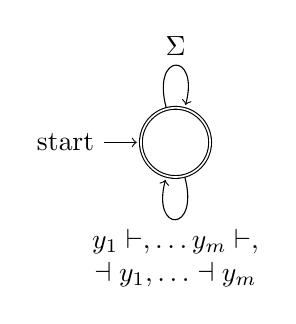
\begin{tikzpicture}[shorten >=1pt,node distance=3cm,on grid,auto]  \node[state,initial,accepting]  (q_0)                      {};  \path[->] (q_0) edge [loop above] node        {$\Sigma$} () 	        edge [loop below] node[align=center]        {$y_{1}\vdash,\ldots y_{m}\vdash,$ \\ $\dashv y_{1},\ldots \dashv y_{m}$} (); \end{tikzpicture}\caption{\label{fig:vset}A vset-automaton $B$ with $\left\llbracket B\right\rrbracket =\Upsilon_{Y}$,
for $Y=\left\{ y_{1},\ldots,y_{m}\right\} $ (this image is taken
from \cite{Fagin:2015:DSF:2772377.2699442}).}
\end{figure}

\begin{example}
Figure \ref{fig:vset} shows a vset-automaton $B$, with $\textrm{SVars}\left(B\right)=Y$,
where $Y=\left\{ y_{1},\ldots,y_{m}\right\} $. We have that $\left\llbracket B\right\rrbracket =\Upsilon_{Y}$.
This shows that vset-automata can express spanners that regex formulas
and vstk-automata cannot. (This example was adapted from \cite{Fagin:2015:DSF:2772377.2699442}).
\end{example}


\subsection{Algebras of Spanners\label{subsec:Algebras-of-Spanners}}

Besides mere span extraction, AQL offers the capability to combine,
transform and filter extracted tuples by using a series of operators.
Here, I introduce the relational operators for spanners, described
in \cite{Fagin:2015:DSF:2772377.2699442}, that are considered to
capture the core relational operations of AQL. They are:
\begin{itemize}
\item \emph{Union }($\cup$);
\item \emph{Projection }($\pi$);
\item \emph{Natural Join} ($\bowtie$);
\item \emph{String Selection} ($\varsigma$).
\end{itemize}
A finite set of spanner operators forms a \emph{spanner algebra}.
In the following, I look at the definitions of the listed spanner
operators.

\subsubsection{Union}

Before giving the definition of the union operator, we need to introduce
the concept of \emph{union compatible spanners.}
\begin{definition}
Given two document spanners $P_{1}$ and $P_{2}$, they are union
compatible if and only if $\textrm{SVars}\left(P_{1}\right)=\textrm{SVars}\left(P_{2}\right)$.
\end{definition}

\noindent The definition of union of two spanners is as follows.
\begin{definition}
Given two union compatible document spanners $P_{1}$ and $P_{2}$,
their union is the spanner denoted as $P_{1}\cup P_{2}$, for which
we have that:

\begin{itemize}
\item $\textrm{SVars}\left(P_{1}\cup P_{2}\right)=\textrm{SVars}\left(P_{1}\right)$;
\item given a string $\mathbf{s}$, $\left(P_{1}\cup P_{2}\right)\left(\mathbf{s}\right)=P_{1}\left(\mathbf{s}\right)\cup P_{2}\left(\mathbf{s}\right)$.
\end{itemize}
\end{definition}


\subsubsection{Projection}
\begin{definition}
Given a document spanner $P$ and a set of span variables $Y\subseteq\textrm{SVars}\left(P\right)$,
the projection of $P$ over $Y$ is the spanner denoted as $\pi_{Y}P$,
satisfying $\textrm{SVars}\left(\pi_{Y}P\right)=Y$.
\end{definition}

\noindent As the name and the definition suggest, the projection of
a document spanner $P$ over a subset of its span variables $Y$ is
obtained by reducing the domain of each of the spanner's output $\mathbf{s}-\textrm{tuples}$
to $Y$.

\subsubsection{Natural Join}
\begin{definition}
Given two document spanners $P_{1}$ and $P_{2}$, their natural join
is the spanner denoted as $P_{1}\bowtie P_{2}$, for which we have
that:

\begin{itemize}
\item $\textrm{SVars}\left(P_{1}\bowtie P_{2}\right)=\textrm{SVars}\left(P_{1}\right)\cup\textrm{SVars}\left(P_{2}\right)$;
\item given a string $\mathbf{s}$, $\left(P_{1}\bowtie P_{2}\right)\left(\mathbf{s}\right)$
consists of all the $\mathbf{s}-\textrm{tuples}$ $\mu$ agreeing
with some $\mu_{1}\in P_{1}\left(\mathbf{s}\right)$ and some $\mu_{2}\in P_{2}\left(\mathbf{s}\right)$.
Note that this implies that $\mu_{1},\mu_{2}$ agree on variables
that are common to $P_{1},P_{2}$: $\forall x\in\textrm{SVars}\left(P_{1}\right)\cap\textrm{SVars}\left(P_{2}\right)$,
$\mu_{1}\left(x\right)=\mu_{2}\left(x\right)$. 
\end{itemize}
\end{definition}

\begin{example}
Consider again the regex formula $\gamma$ from Example \ref{ex-rgx}.
The reader can verify that $\gamma$ can be expressed as:

\ldots{}
\begin{equation}
\left(\Sigma^{\ast}\cdot x\left\{ \gamma_{action}\right\} \cdot\Sigma^{\ast}\right)\bowtie\left(\Sigma^{\ast}\cdot y\left\{ \gamma_{title}\right\} \cdot\Sigma^{\ast}\right)\bowtie\left(\Sigma^{\ast}\cdot z\left\{ x\left\{ \Sigma^{+}\right\} \cdot\Sigma^{+}\cdot y\left\{ \Sigma^{+}\right\} \right\} \cdot\Sigma^{\ast}\right)
\end{equation}
.
\end{example}


\subsubsection{String Selection}
\begin{definition}
Given a document spanner $P$ and a k-ary string relation $R$, the
string selection operation according to $R$ is denoted as $\varsigma^{R}$,
and is parametrized by $x_{1},...,x_{k}\in\textrm{SVars}\left(P\right)$.
We have that, given a string $\mathbf{s}$ and a spanner $P':=\varsigma_{x_{1},...,x_{k}}^{R}P$,
$P'\left(\mathbf{s}\right)$ consists of all the $\mathbf{s}-\textrm{tuples}$
$\mu$ such that $\left(\mathbf{s}_{\mu\left(x_{1}\right)},...,\mathbf{s}_{\mu\left(x_{k}\right)}\right)\in R$.
\end{definition}

\noindent In the remainder of this document, the only string selection
operator I consider is $\varsigma_{x,y}^{=}$ which, given a spanner
$P$, restricts $P\left(\mathbf{s}\right)$ to those $\mathbf{s}-\textrm{tuples}$
that satisfy $\mathbf{s}_{\mu\left(x\right)}=\mathbf{s}_{\mu\left(y\right)}$.

\medskip{}

\noindent I now introduce some additional notation. Given a generic
class of spanner representations $\textrm{SR}$, the set of all the
spannners that can be represented by $\textrm{SR}$ is denoted as
$\left\llbracket \textrm{SR}\right\rrbracket $. Formally, we have
that $\left\llbracket \textrm{SR}\right\rrbracket =\left\{ \left\llbracket r\right\rrbracket \mid r\in\textrm{SR}\right\} $.
Let $O$ be a spanner algebra. I denote by $\textrm{SR}^{O}$ the
closure of $\textrm{SR}$ under $O$, that is: the class of spanner
represantations obtained by applying (compositions of) operators contained
in $O$ to the represantations in $\textrm{SR}$. The corresponding
set of spanners is referred to as $\left\llbracket \textrm{SR}^{O}\right\rrbracket $.
We are ready to start reasoning on the expressive power of the spanner
representations that we saw. Please refer to \cite{Fagin:2015:DSF:2772377.2699442}
for the proofs of the mathematical statements in the remainder of
this Chapter.
\begin{proposition}
The following hold:

\begin{enumerate}
\item every document spanner represented in the classes $\textrm{RGX}$
and $\textrm{VA}_{\textrm{stk}}$ is hierarchical, that is: $\left\llbracket \textrm{\textrm{RGX}}\right\rrbracket ,\left\llbracket \textrm{\ensuremath{\textrm{VA}_{\textrm{stk}}}}\right\rrbracket \subseteq\mathbf{HS}$;
\item there exist some spanners represented in $\textrm{VA}_{\textrm{set}}$
that are not hierarchical: $\left\llbracket \textrm{\ensuremath{\textrm{VA}_{set}}}\right\rrbracket \nsubseteq\mathbf{HS}$;
\item the operators $\cup$, $\pi$, $\varsigma^{R}$ preserve the property
of being hierarchical, while $\bowtie$ does not, thus we have that:

\begin{enumerate}
\item given a class of spanner representations $\textrm{SR}$, $\left\llbracket \textrm{SR}\right\rrbracket \subseteq\mathbf{HS}\Rightarrow\left\llbracket \textrm{SR}^{\left\{ \cup,\pi,\varsigma^{R}\right\} }\right\rrbracket \subseteq\mathbf{HS};$
\item there exist two hierarchical spanners $P_{1},P_{2}$ such that $P_{1}\bowtie P_{2}\notin\mathbf{HS}$.
\end{enumerate}
\end{enumerate}
\end{proposition}

\noindent In the next Subsection, I discuss the class of \emph{regular
spanners}, which plays a central role in the construction of the class
of spanners constituting the core of AQL.

\subsection{Regular Spanners}

A regular spanner is defined as follows.
\begin{definition}
A spanner is regular if it can be defined by a vset-automaton.
\end{definition}

\noindent Let us see how regular spanners are related to the other
basic spanner classes. A preliminary result is that regex formulas
and vstk-automata have the same expressive power.
\begin{theorem}
\label{.rgx=00003Dvstk}$\left\llbracket \textrm{\textrm{RGX}}\right\rrbracket =\left\llbracket \textrm{\ensuremath{\textrm{VA}_{\textrm{stk}}}}\right\rrbracket $.
\end{theorem}

\noindent It turns out that the spanners expressed by representations
in $\textrm{\ensuremath{\textrm{VA}_{\textrm{stk}}}}$($\textrm{\textrm{RGX}}$)
are exactly those that are both regular and hierarchical.
\begin{theorem}
$\left\llbracket \textrm{\ensuremath{\textrm{VA}_{\textrm{stk}}}}\right\rrbracket =\left\llbracket \textrm{\ensuremath{\textrm{VA}_{\textrm{set}}}}\right\rrbracket \cap\mathbf{HS}$.
\end{theorem}

\noindent For what concerns the algebraic operators I presented in
Subsection \ref{subsec:Algebras-of-Spanners}, it can be shown that
union, projection and join don't increase the expressive power of
regular spanners.
\begin{theorem}
\label{.setext=00003Dset}$\left\llbracket \textrm{\ensuremath{\textrm{VA}_{\textrm{set}}}}^{\left\{ \cup,\pi,\bowtie\right\} }\right\rrbracket =\left\llbracket \textrm{\ensuremath{\textrm{VA}_{\textrm{set}}}}\right\rrbracket $.
\end{theorem}

\noindent On the other hand, applying the same operators to the spanner
representations in $\textrm{\ensuremath{\textrm{VA}_{\textrm{stk}}}}$
results in a class equivalent to regular spanners.
\begin{theorem}
\label{.stkext=00003Dset}$\left\llbracket \textrm{\ensuremath{\textrm{VA}_{\textrm{stk}}}}^{\left\{ \cup,\pi,\bowtie\right\} }\right\rrbracket =\left\llbracket \textrm{\ensuremath{\textrm{VA}_{\textrm{set}}}}\right\rrbracket $.

\medskip{}
\end{theorem}

\noindent Let us now look at which string relations can be simulated
by regular spanners, starting with the concept of \emph{selectable
string relation}.
\begin{definition}
Given a string relation $R$ and a class of spanners $C$, $R$ is
selectable by $C$ if for every document spanner $P\in C$ and for
every $\overrightarrow{x}=x_{1},...,x_{k}$, $x_{i}\in\textrm{SVars}\left(P\right)$,
we have that $\varsigma_{\overrightarrow{x}}^{R}P\in C$.
\end{definition}

\noindent Next, I introduce the concept of \emph{restricted universal
spanner.}
\begin{definition}
Given a string relation $R$ and a sequence of variables$\overrightarrow{x}=x_{1},...,x_{k}$
with their corrsesponding set $X=\left\{ x_{1},...,x_{k}\right\} $,
the $R-\textrm{restricted}$ universal spanner over $\overrightarrow{x}$
is $\Upsilon_{\overrightarrow{x}}^{R}:=\varsigma_{\overrightarrow{x}}^{R}\Upsilon_{X}$.
\end{definition}

\noindent Selectability of a string relation $R$ by a class of spanners
$C$ corresponds to the presence in $C$ of all the possible $R-\textrm{restricted}$
universal spanners, under some conditions.
\begin{proposition}
Given a string relation $R$ and a class of spanners $C$ containing
all the possible universal spanners and closed under natural join,
$R$ is selectable by $C$ if and only if, for every $\overrightarrow{x}=x_{1},...,x_{k}\in\textrm{SVars}^{k}$,
$\Upsilon_{\overrightarrow{x}}^{R}\in C$.
\end{proposition}

\noindent In the case of regular spanners, the class of string relations
that they can select is exactly $\textrm{REC}$.
\begin{theorem}
The class of string relations selectable by $\left\llbracket \textrm{\ensuremath{\textrm{VA}_{\textrm{set}}}}\right\rrbracket $
is $\textrm{REC}$.
\end{theorem}

\noindent The relation ``$=$'' is not in $\textrm{REC}$, thus
it is not selectable by regular spanners, nonetheless it is important
for selection predicates in AQL, which is why regular spanners don't
have enough expressive power to model its core. In the following Subsection,
I describe the spanners that are identified in \cite{Fagin:2015:DSF:2772377.2699442}
as the core of AQL: \emph{core spanners}.

\subsection{Core Spanners}

An expression in the core of AQL belongs to $\textrm{RGX}^{\left\{ \cup,\pi,\bowtie,\varsigma^{=}\right\} }$.
Consequently, a core spanner is defined as follows.
\begin{definition}
\label{core-def}A core spanner is a document spanner belonging to
$\left\llbracket \textrm{RGX}^{\left\{ \cup,\pi,\bowtie,\varsigma^{=}\right\} }\right\rrbracket $.
\end{definition}

\noindent Thanks to Theorems \ref{.rgx=00003Dvstk}, \ref{.setext=00003Dset}
and \ref{.stkext=00003Dset} we can easily state the next theorem. 
\begin{theorem}
\noindent \label{RGX=00003DSET}$\left\llbracket \textrm{RGX}^{\left\{ \cup,\pi,\bowtie,\varsigma^{=}\right\} }\right\rrbracket =\left\llbracket \textrm{\ensuremath{\textrm{VA}_{\textrm{stk}}}}^{\left\{ \cup,\pi,\bowtie,\varsigma^{=}\right\} }\right\rrbracket =\left\llbracket \textrm{\ensuremath{\textrm{VA}_{\textrm{set}}}}^{\left\{ \cup,\pi,\bowtie,\varsigma^{=}\right\} }\right\rrbracket $. 
\end{theorem}

\noindent This shows that core spanners can be reduced to regular
spanners extended with the algebra $\left\{ \cup,\pi,\bowtie,\varsigma^{=}\right\} $.
But the following lemma tells us an algebra with fewer operators is
also sufficient.
\begin{lemma}
$\left\llbracket \textrm{\ensuremath{\textrm{VA}_{\textrm{set}}}}^{\left\{ \cup,\pi,\bowtie,\varsigma^{=}\right\} }\right\rrbracket =\left\llbracket \textrm{\ensuremath{\textrm{VA}_{\textrm{set}}}}^{\left\{ \pi,\varsigma^{=}\right\} }\right\rrbracket $.
\end{lemma}

\noindent Another lemma, known as the \emph{core simplification lemma},
gives an even more simple way of representing core spanners.
\begin{lemma}
\label{Core-simplif}$\mathbf{(Core\,Simplification\,Lemma)}$ Every
core spanner can be defined by an expression of the form

\begin{equation}
\pi_{V}SA
\end{equation}

\noindent where:

\begin{itemize}
\item $A$ is a vset-automaton;
\item $V\subseteq\textrm{SVars}\left(A\right)$;
\item $S$ is a sequence of string selections $\varsigma_{x,y}^{=}$, for
$x,y\in\textrm{SVars}\left(A\right)$.
\end{itemize}
\end{lemma}

\noindent For what concerns which string relations can be simulated
by core spanners, the next definition presents three string relations
of relevance.
\begin{definition}
Given two strings $\mathbf{s},\mathbf{t}\in\varSigma^{\ast}$:

\begin{itemize}
\item $\mathbf{s}\sqsubseteq\mathbf{t}$ if $\mathbf{s}$ is a (consecutive)
substring of t (i.e. $\mathbf{s}=\mathbf{t}_{\left[i,j\right\rangle }$);
\item $\mathbf{s}\sqsubseteq_{\textrm{prf}}\mathbf{t}$ if $\mathbf{s}$
is a prefix of t (i.e. $\mathbf{s}=\mathbf{t}_{\left[1,j\right\rangle }$);
\item $\mathbf{s}\sqsubseteq_{\textrm{sfx}}\mathbf{t}$if $\mathbf{s}$
is a suffix of t (i.e. $\mathbf{s}=\mathbf{t}_{\left[1,\left|\mathbf{t}\right|+1\right\rangle }$).
\end{itemize}
\end{definition}

\begin{proposition}
\noindent All the string relations in $\textrm{REC}$, $\mathbf{\sqsubseteq}$,
$\sqsubseteq_{\textrm{prf}}$ and $\sqsubseteq_{\textrm{sfx}}$ are
selectable by the core spanners.
\end{proposition}


\subsection{Difference}

The difference operator is defined as follows.
\begin{definition}
Given two union compatible document spanners $P_{1}$ and $P_{2}$,
their difference is the spanner $P_{1}\setminus P_{2}$, for which
we have:

\begin{itemize}
\item $\textrm{SVars}\left(P_{1}\setminus P_{2}\right)=\textrm{SVars}\left(P_{1}\right)$;
\item given a string $\mathbf{s}$, $\left(P_{1}\setminus P_{2}\right)\left(\mathbf{s}\right)=\left(P_{1}\right)\setminus\left(P_{2}\right)\left(\mathbf{s}\right)$.
\end{itemize}
\end{definition}

\noindent It can be shown that regular spanners are closed under difference.
\begin{theorem}
\label{.setdiff=00003Dset}$\left\llbracket \textrm{\ensuremath{\textrm{VA}_{\textrm{set}}}}^{\left\{ \setminus\right\} }\right\rrbracket =\left\llbracket \textrm{\ensuremath{\textrm{VA}_{\textrm{set}}}}\right\rrbracket $.
\end{theorem}

\noindent Despite the result of of Theorem \ref{.setdiff=00003Dset},
core spanners are not closed under difference, which is why this operator
has not been considered so far.
\begin{theorem}
\label{.last-stat}$\left\llbracket \textrm{RGX}^{\left\{ \cup,\pi,\bowtie,\varsigma^{=}\right\} }\right\rrbracket \subsetneq\left\llbracket \textrm{RGX}^{\left\{ \cup,\pi,\bowtie,\varsigma^{=},\setminus\right\} }\right\rrbracket $.
\end{theorem}


\chapter{A Runtime System for AQL's Core}

In this chapter I describe a new runtime system for AQL's core fragments.
It is based on a modified version of vset-automata, the \emph{extended
vset-automata (}or \emph{eVset-automata).} In particular, the system
works with a particular kind of eVset-automata: \emph{well-behaved
eVset-automata. }I start by defining eVset-automata, then I describe
well-behaved eVset-automata and their properties, with particular
attention to their ability to support the operations from the algebra
presented in Subsection \ref{subsec:Algebras-of-Spanners}. Subsequently,
I review some interesting ways of running usual nondeterministic automata
on a string, from which I took inspiration for my implementation.
Finally I explain how the system works.

\section{Extended Vset-automata}

Before I define extended vset-automata formally, I introduce some
basic concepts.
\begin{definition}
Given a set $X\subseteq\textrm{SVars}$, we define:

\begin{itemize}
\item $\textrm{SVOps}^{\vdash}\left(X\right)=\left\{ x\vdash\mid x\in X\right\} $;
\item $\textrm{SVOps}^{\dashv}\left(X\right)=\left\{ \dashv x\mid x\in X\right\} $;
\item $\textrm{SVOps}\left(X\right)=\textrm{SVOps}^{\vdash}\left(X\right)\cup\textrm{SVOps}^{\dashv}\left(X\right)$.
\end{itemize}
\end{definition}

\noindent I now define an extended vset-automaton.
\begin{definition}
An extended \emph{variable-set automaton} (or \emph{eVset-automaton})
is a tuple $\left(Q,q_{0},q_{f},\delta\right)$, where:

\begin{itemize}
\item $Q$ is a finite set of states;
\item $q_{0}\in Q$ is the initial state;
\item $q_{f}\in Q$ is the accepting state;
\item $\delta=\delta^{\textrm{char}}\cup\delta^{\textrm{op}}$ is a finite
transition relation consisting of triples, where:

\begin{itemize}
\item $\delta^{\textrm{char}}=\left\{ \left(q,\sigma,q'\right)\mid q,q'\in Q,\sigma\in\varSigma\right\} $,
whose elments are called character transitions;
\item $\delta^{\textrm{op}}=\left\{ \left(q,S,q'\right)\mid q,q'\in Q,S\subseteq\textrm{SVOps\ensuremath{\left(SVars\right)}}\right\} $,
whose elements are called operation transitions .
\end{itemize}
\end{itemize}
\end{definition}

\noindent In a transition$\left(q,a,q'\right)$ with label $a$ from
state $q$ to state $q'$, $q$ is called the \emph{source state},
while $q'$ is called the \emph{destination state}. By a slight abuse
of notation, I denote by $\textrm{SVOps}\left(A\right)$ the set of
variable operations appearing in the transitions of an eVset-automaton
$A$. $\textrm{SVars}\left(A\right)$ is defined as for a usual vset-automaton.
I now define a configuration and, subsequently, a run of an eVset-automaton.
\begin{definition}
Given a string $\mathbf{s}$, $\left|\mathbf{s}\right|=n$, and an
eVset-automaton $A=\left(Q,q_{0},q_{f},\delta\right)$, a configuration
of A is a tuple $c=\left(q,V,Y,i\right)$, where:

\begin{itemize}
\item $q\in Q$ is the current state;
\item $V\subseteq\textrm{SVars}\left(A\right)$ is the active variable set;
\item $Y\subseteq\textrm{SVars}\left(A\right)$ is the set of available
variables;
\item $i$ is an index belonging to $\left\{ 1,\ldots,n+1\right\} $.
\end{itemize}
\end{definition}

\begin{definition}
\label{e-run}Given a string $\mathbf{s}=s_{1},\ldots,s_{n}$ and
an eVset-automaton $A=\left(Q,q_{0},q_{f},\delta\right)$, a run $\rho$
of $A$ on $\mathbf{s}$ is a sequence $c_{0},\ldots,c_{m}$ of configurations,
where:

\begin{itemize}
\item $c_{0}=\left(q_{0},\textrm{�},\textrm{SVars}\left(A\right),1\right)$;
\item for $j=0,\ldots,m-1$ one of the following holds for $c_{j}=\left(q_{j},V_{j},Y_{j},i_{j}\right)$
and $c_{j+1}=\left(q_{j+1},V_{j+1},Y_{j+1},i_{j+1}\right)$:

\begin{itemize}
\item $V_{j+1}=V_{j}$, $Y_{j+1}=Y_{j}$, $i_{j+1}=i_{j}+1$ and $\left(q_{j},s_{j}q_{j+1}\right)\in\delta^{\textrm{char}}$;
\item $i_{j+1}=i_{j}$, and for some $S\subseteq\textrm{SVOps}\left(A\right)$
we have :

\begin{itemize}
\item for each $x\in\textrm{SVars}\left(A\right)$:

\begin{itemize}
\item $\left\{ x\vdash,\dashv x\right\} \cap S=\left\{ x\vdash\right\} $
or $\left\{ x\vdash,\dashv x\right\} \cap S=\left\{ x\vdash,\dashv x\right\} $
if and only if $x\in Y_{j}$;
\item $\left\{ x\vdash,\dashv x\right\} \cap S=\left\{ \dashv x\right\} $
if and only if $x\in V_{j}$;
\end{itemize}
\item $V_{j+1}=V_{j}\cup\left\{ x\mid x\vdash\in S\right\} \setminus\left\{ x\mid\dashv x\in S\right\} $;
\item $Y_{j+1}=Y_{j}\setminus\left\{ x\mid x\vdash\in S\right\} $;
\item $\left(q_{j},S,q_{j+1}\right)\in\delta^{\textrm{op}}$.
\end{itemize}
\end{itemize}
\end{itemize}
$\rho$ is accepting if $c_{m}=\left(q_{f},\textrm{�,}\textrm{�},n+1\right)$.
\end{definition}

$\textrm{ARuns}\left(A,\mathbf{s}\right)$ and $\left\llbracket A\right\rrbracket $,
for an eVset-automaton $A$ and a string $\mathbf{s}$, are defined
in similar ways to those of usual vset-automata. This new kind vset-automata
allows to perform an arbitrary number of variable operations in one
transition. The operations in a transition are to be performed in
a given order. The exact order isn't very important, except for the
fact that, in a valid run, the insertion and removal of a variable
from the active variable set need to happen in the correct order (i.e.
insertion first). 

\begin{figure}
\centering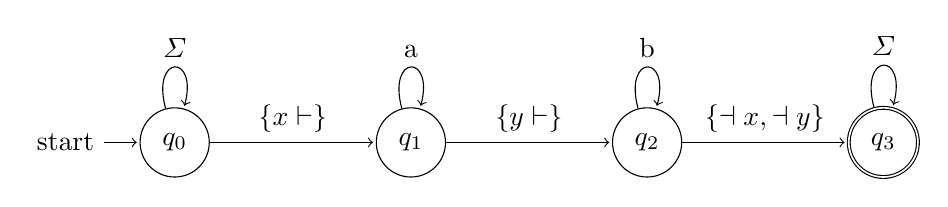
\begin{tikzpicture}[shorten >=1pt,node distance=3cm,on grid,auto] \node[state,initial]  (q_0)                      {$q_0$}; \node[state]          (q_1) [right=of q_0] {$q_1$}; \node[state]          (q_2) [right=of q_1] {$q_2$}; \node[state,accepting](q_3) [right=of q_2] {$q_3$}; \path[->] (q_0) edge              node        {$\left\{ x\vdash\right\} $} (q_1) 		edge [loop above] node        {$\varSigma$} () 	  (q_1) edge 	          node        {$\left\{ y\vdash\right\} $} (q_2) 		edge [loop above] node        {a} (q_2) 	  (q_2) edge              node        {$\left\{ \dashv x,\dashv y\right\} $} (q_3) 		edge [loop above] node        {b} () 	  (q_3) edge [loop above] node        {$\varSigma$} (); \end{tikzpicture}

\caption{\label{fig:evset}An eVset-automaton $A$.}
\end{figure}

The reason for using eVset-automata instead of plain vset-automata
will be clear in the next section. I now introduce some additional
useful concepts, the most important of which being that of a \emph{path}
in an eVset-automaton.
\begin{definition}
Given a transition $t\in\delta$ in an eVset-automaton $A$, and an
ordering $\varphi$ on the elements of $\textrm{SVOps}\left(A\right)$,
we define

\begin{itemize}
\item $\textrm{Ops}\left(t\right)$as either:

\begin{itemize}
\item if $t=\left(q,S,q'\right)\in\delta^{\textrm{op}}$, the set $S$;
\item if $t\in\delta^{\textrm{char}}$, the empty set.
\end{itemize}
\item $\textrm{LOps}_{\varphi}\left(t\right)$ as either:

\begin{itemize}
\item if $t=\left(q,S,q'\right)\in\delta^{\textrm{op}}$, the list $o_{1},\ldots,o_{\left|S\right|}$
of operations belonging to $S$, ordered according to $\varphi$;
\item if $t\in\delta^{\textrm{char}}$, the empty list.
\end{itemize}
\end{itemize}
\end{definition}

\begin{definition}
\noindent Given an extended vset-automaton $A=\left(Q,q_{0},q_{f},\delta\right)$
and a pair of states $q,q'\in Q$, a path $p$ between $q$ and $q'$
in $A$ is a sequence of transitions $t_{1},$$\ldots,t_{n}\in\delta$,
such that:

\begin{itemize}
\item the source state of $t_{1}$ is $q$;
\item the destination state of $t_{n}$ is $q'$;
\item for every pair $t_{i},t_{i+1}$, the destination state of $t_{i}$
equals the source state of $t_{i+1}$.
\end{itemize}
We also write $p_{q}^{q'}$. We refer to the set of paths in $A$
as $\textrm{Paths}\left(A\right)$.
\end{definition}

A path in an eVset-automaton is closely related to a run, as formalized
by the next definition.
\begin{definition}
Given a string $\mathbf{s}$, an eVset-automaton $A=\left(Q,q_{0},q_{f},\delta\right)$,
a run $\rho=c_{0},$$\ldots,c_{m}$ of $A$ on $\mathbf{s}$ and a
path $p=t_{0},\ldots,t_{m-1}$ in $A$, we say that $p$ supports
$\rho$ if, for every pair $c_{i}$, $c_{i+1}$ of configurations,
$c_{i+1}$is obtained from $c_{i}$ by applying $t_{i}$, using the
rules given in Definition \ref{e-run}.
\end{definition}

\begin{definition}
Given a path $p=t_{1},\ldots,t_{n}$ in an eVset-automaton $A$, and
considering an ordering $\varphi$ on the elements of $\textrm{SVOps}\left(A\right)$,
we define

\begin{itemize}
\item the set $\textrm{Ops}\left(p\right)$ as
\[
\bigcup_{i=1}^{n}\textrm{Ops}\left(t_{i}\right)
\]
\item the list $\textrm{LOps}_{\varphi}\left(p\right)$ as
\[
\bigoplus_{i=1}^{n}\textrm{LOps}_{\varphi}\left(t_{i}\right)
\]
where $\bigoplus$ is the usual list concatenation operator.
\end{itemize}
If every transition in $p$ belongs to $\delta^{\textrm{op}}$, we
say that $p$ is an operation-only path.
\end{definition}

From now on, without loss of generality, I consider a fixed order
$\varphi$, in which insertions come before deletions.

\medskip{}

As shown in the previous chapter, the class of vset-automata doesn't
get more expressive power when extended with the algebra$\left\{ \cup,\pi,\bowtie\right\} $.
Hence, this class is a good candidate to be the base for a class of
representations for the core spanners, as the Core Simplification
Lemma suggests. In the following, I show that the same result holds
for a subclass of extended vset-automata: \emph{well-behaved eVset-automata}.
Moreover, we will see that an AQL core fragment, as defined in \cite{Fagin:2015:DSF:2772377.2699442},
can be converted into a well-behaved eVset-automaton. The runtime
system implicitly assumes that any eVset-automaton it receives as
input is well-behaved.

\section{Well-Behaved Extended Vset-Automata}

In order to be well-behaved, an eVset-automaton has to respect some
constraints on its paths that are between its initial and accepting
state. I call this kind of paths \emph{complete paths.}
\begin{definition}
\noindent Given an eVset-automaton $A=\left(Q,q_{0},q_{f},\delta\right)$,
a path $p=t_{1},\ldots,t_{n}$ in $A$ is complete if it is between
$q_{0}$ and $q_{f}$, that is $p=p_{q_{0}}^{q_{f}}$.
\end{definition}

I now formally define a well-behaved eVset-automaton.
\begin{definition}
\noindent \label{well-behaved}An eVset-automaton $A$ is well-behaved
if, for every complete path $p$ in $A$ we have:

\begin{enumerate}
\item for every $o\in\textrm{SVOps}\left(A\right)$, $o$ appears exactly
once in $\textrm{LOps}\left(p\right)$;\label{enu:well-behaved-1,}
\item for every pair of operations $x\vdash$,$\dashv x$$\in\textrm{SVOps}\left(A\right)$,
$x\vdash$ appears before $\dashv x$ in $\textrm{LOps}\left(p\right)$.
\end{enumerate}
\end{definition}

According to the definition, well-behaved eVset-automata guarantee
that any of their complete paths will support a valid accepting run.
Since states that cannot reach the final state, or that cannot be
reached from the initial state, are not used in complete paths, we
might want to consider only well-behaved eVset-automata where these
states don't exist.
\begin{definition}
Given an eVset-automaton $A$, $A$ is pruned if for every state $q$
in $A$, there is a path from $q_{0}$ to $q$, and a path from $q$
to $q_{f}$ in $A$.
\end{definition}

\begin{example}
The eVset automaton $A$ from Figure \ref{fig:evset} and the eVset-automaton
$B$ from Figure \ref{evset-2} are well-behaved and pruned.
\end{example}

The next proposition tells us that the we can always prune a well-behaved
eVset-automaton, obtaining a new eVset-automaton equivalent to the
original.
\begin{proposition}
Given a well-behaved eVset-automaton $A$, there exists a pruned well-behaved
eVset automaton $A'$ such that $\left\llbracket A'\right\rrbracket =\left\llbracket A\right\rrbracket $.
Moreover, $A'$ can be produced in polynomial time.
\end{proposition}

\begin{proof}
To obtain $A'$, it is sufficient to remove from $A$ those states
from which we can't reach the final state, those states that are unreachable
from the initial state, and all the transitions that have them as
source or destination states. To test each state for removal we can
use, e. g., Dijkstra's shortest path algorithm, which ensures $A'$
can be found in polynomial time. Because of our construction, $A'$
is well-behaved, as all its complete paths are also in $A$. We now
show that, for every string $\mathbf{s},$ we have $\left\llbracket A'\right\rrbracket \left(\mathbf{s}\right)=\left\llbracket A\right\rrbracket \left(\mathbf{s}\right)$.
To see that $\left\llbracket A'\right\rrbracket \left(\mathbf{s}\right)\subseteq\left\llbracket A\right\rrbracket \left(\mathbf{s}\right)$,
we can notice that each run $\rho'$ of $A'$ on $\mathbf{s}$ that
is accepting can be supported only by a complete path $p'$, which
is also in $A$ by construction. $\left\llbracket A\right\rrbracket \left(\mathbf{s}\right)\subseteq\left\llbracket A'\right\rrbracket \left(\mathbf{s}\right)$
is true as well because we include in $A'$ all the complete paths
existing in $A$ so every run $p$ of $A$ on $\mathbf{s}$ is also
a run of $A'$.
\end{proof}

If a well-behaved eVset-automaton is pruned, it automatically gets
two other properties.
\begin{corollary}
Given a pruned well-behaved eVset-automaton $A$, for every path$p$
in $A$ $\textrm{LOps}\left(p\right)$ contains no duplicates.
\end{corollary}

\begin{proof}
Since $A$ is pruned, $p$ is part of a complete path $p'$. But $A$
is also well-behaved, so $\textrm{LOps}\left(p'\right)$ contains
no duplicates, which implies that $\textrm{LOps}\left(p\right)$ has
no duplicates either.
\end{proof}

\begin{corollary}
\label{same-ops}Given a pruned well-behaved eVset-automaton $A$,
and two states $q,q'$ in $A$, for every pair of paths $p,p'$ between
$q$ and $q'$ in $A$, $\textrm{Ops}\left(p\right)=\textrm{Ops}\left(p'\right)$.
\end{corollary}

\begin{proof}
Since $A$ is pruned, there surely exists a path $p^{0}$ between
$q_{0}$ and $q$. For the same reason, there exists a path $p^{f}$
between $q'$ and $q_{f}$. So $q$ and $q'$ appear in two complete
paths, which we may call $p^{0}pp^{f}$ and $p^{0}p'p^{f}$, that
differ only in the subpaths between $q$ and $q'$. If $\textrm{Ops}\left(p\right)\neq\textrm{Ops}\left(p'\right)$,
then one of $p^{0}pp^{f}$ and $p^{0}p'p^{f}$ wouldn't satisfy the
requirement \ref{enu:well-behaved-1,} of \ref{well-behaved}, making
$A$ not well-behaved, a contraddiction.
\end{proof}

\medskip{}

In the following, I describe the constructions that I use in my system
to support algebraic operations with well-behaved eVset-automata.
The main advantage of these constructions is that they produce a well-behaved
eVset-automaton whose size is \emph{polynomial} in the size of the
input automaton/a. Let us start with projection.

\begin{theorem}
\noindent \label{ext-proj}Given a well-behaved eVset-automaton $A$,
the set $X=\textrm{SVars}\left(A\right)$ and a set $Y\subseteq X$,
a well behaved eVset-automaton $A'$ can be produced in linear time
such that $\left\llbracket A'\right\rrbracket =\pi_{Y}\left\llbracket A\right\rrbracket $.
\end{theorem}

\begin{proof}
Let us consider $A=\left(Q,q_{0},q_{f},\delta\right)$. We can take
$A'=\left(Q',q_{0}',q_{f}',\delta'\right)$, where:

\begin{itemize}
\item $Q'=Q$;
\item $q_{0}'=q_{0}$;
\item $q_{f}'=q_{f}$;
\item $\delta'=\left(\delta\setminus\delta^{\textrm{unprojected}}\right)\cup\delta^{\textrm{projected}}$,
where:

\begin{itemize}
\item $\delta^{\textrm{unprojected}}=\left\{ \left(q,S,q'\right)\in\delta\mid S\cap\textrm{SVOps}\left(X\setminus Y\right)\neq\textrm{�}\right\} $;
\item $\delta^{\textrm{projected}}=\left\{ \left(q,S',q'\right)\mid\exists\left(q,S,q'\right)\in\delta^{\textrm{unprojected}}:S'=S\setminus\textrm{SVOps}\left(X\setminus Y\right)\right\} $.
\end{itemize}
\end{itemize}
This construction removes all the occurencies of variable operations
concerning variables excluded from the projection from the transitions
of $A$. $A'$ is still well-behaved, since we maintain the occurrencies
of operations concerning the variables on which we project, that continue
to appear exactly once on each path, and in the right order. Assuming
the size of $A$, that we may call $n$, as the sum of the sizes of
$Q$, $\delta$ and $\textrm{SVars}\left(A\right)$, it is easy to
verify that this construction can be carried out in $O\left(n\right)$.
Let us show that $\left\llbracket A'\right\rrbracket =\pi_{Y}\left\llbracket A\right\rrbracket $.
Notice that given a string $\mathbf{s}$, for each accepting run $\rho$
of $A$ on $\mathbf{s}$, producing an $\mathbf{s}$-tuple $\mu$,
there is an accepting run $\rho'$ of $A'$ that produces an $\mathbf{s}$-tuple
$\mu'$, which assigns the same spans as $\mu$ to the variables in
common with $\mu'$, which by construction belong to $Y$. The path
$p'$ supporting $\rho'$ is exactly the path obtained by modifying
the path $p$, that supports $\rho$, by eliminating the operations
on unprojected variables. This shows that $\pi_{Y}\left\llbracket A\right\rrbracket \subseteq\left\llbracket A'\right\rrbracket $.
It must also be that $\left\llbracket A'\right\rrbracket \subseteq\pi_{Y}\left\llbracket A\right\rrbracket $,
because no additional complete paths were added to $A'$.
\end{proof}

A similar result holds for the union operation.

\begin{theorem}
\noindent \label{ext-union}Given two well-behaved eVset-automata
$A$ and $B$ that are union-compatible, a third well-behaved eVset-automaton
$C$ can be produced in linear time such that $\left\llbracket C\right\rrbracket =\left\llbracket A\right\rrbracket \cup\left\llbracket B\right\rrbracket $.
\end{theorem}

\begin{proof}
Let us consider $A$ to be of the form $\left(Q^{A},q_{0}^{A},q_{f}^{A},\delta^{A}\right)$
and $B$ of the form $\left(Q^{B},q_{0}^{B},q_{f}^{B},\delta^{B}\right)$.
We can take $C=\left(Q^{C},q_{0}^{C},q_{f}^{C},\delta^{C}\right)$,
where:

\begin{itemize}
\item $Q^{C}=Q^{A}\cup Q^{B}\cup\left\{ q_{0}^{C},q_{f}^{C}\right\} $;
\item $\delta^{C}=\delta^{A}\cup\delta^{B}\cup\left\{ \left(q_{0}^{C},\textrm{�},q_{0}^{B}\right),\left(q_{f}^{B},\textrm{�},q_{f}^{C}\right),\left(q_{0}^{C},\textrm{�},q_{0}^{A}\right),\left(q_{f}^{A},\textrm{�},q_{f}^{C}\right)\right\} $.
\end{itemize}
In this construction, we allow to go from the initial state of $C$
to the initial state of either $A$ or $B$, and to go from the accepting
state of $A$ or that of $B$ to the one of $C$, without any new
variable operations. Thus, given a string $\mathbf{s}$, $C$ can
span exactly the $\mathbf{s}-$tuples contained in $\left\llbracket A\right\rrbracket \left(\mathbf{s}\right)\cup\left\llbracket B\right\rrbracket \left(\mathbf{s}\right)$.
Regarding the complexity of the construction, the operations that
we perform here are the union of the states sets and transition functions,
with the addition of a fixed number of new transitions and states.
Let us consider the size of the input as $n=n_{A}+n_{B}=\left|Q^{A}\right|+\left|\delta^{A}\right|+\left|\textrm{SVars}\left(A\right)\right|+\left|Q^{B}\right|+\left|\delta^{B}\right|+\left|\textrm{SVars}\left(B\right)\right|$.
If we assume the costs of basic operations, as adding/deleting a state/transitions,
to be constant, then obtaining $Q^{C}$ takes $O\left(\left|Q^{B}\right|\right)=O\left(n\right)$
time, and constructing $\delta^{C}$ takes $O\left(\left|\delta^{B}\right|\right)=O\left(n\right)$
time.
\end{proof}

In order to show that we can obtain the natural join of two spanners,
represented by well-behaved eVset-automata, so that the size of the
correspondent resulting eVset-automaton is polynomial in the size
of the input automata, we need a few more steps with respect to the
previous cases. The construction that I present is conceptually very
similar to that described in \cite{Fagin:2015:DSF:2772377.2699442}
for the natural join of plain vset-automata. That construction simulates
running the input automata in parallel, making sure that operations
on common variables are performed simultaneously. Unfortunately this
doesn't work in general, as the next example shows.

\begin{figure}
\centering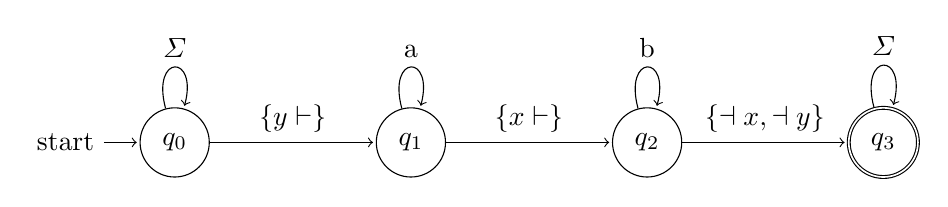
\begin{tikzpicture}[shorten >=1pt,node distance=3cm,on grid,auto] \node[state,initial]  (q_0)                      {$q_0$}; \node[state]          (q_1) [right=of q_0] {$q_1$}; \node[state]          (q_2) [right=of q_1] {$q_2$}; \node[state,accepting](q_3) [right=of q_2] {$q_3$}; \path[->] (q_0) edge              node        {$\left\{ y\vdash\right\} $} (q_1) 		edge [loop above] node        {$\varSigma$} () 	  (q_1) edge 	          node        {$\left\{ x\vdash\right\} $} (q_2) 		edge [loop above] node        {a} (q_2) 	  (q_2) edge              node        {$\left\{ \dashv x,\dashv y\right\} $} (q_3) 		edge [loop above] node        {b} () 	  (q_3) edge [loop above] node        {$\varSigma$} (); \end{tikzpicture}

\caption{\label{evset-2}An eVset-automaton $B$.}

\end{figure}

\begin{example}
Consider the eVset-automaton $A$ from Figure \ref{fig:evset}, the
eVset-automaton $B$ from Figure \ref{evset-2} and the string $\mathbf{s}=$'b'.
$\left\llbracket A\right\rrbracket \left(\mathbf{s}\right)$ contains
the $\mathbf{s}$-tuple $\mu$ such that $\mu\left(x\right)=\left[0,0\right\rangle $
and $\mu\left(y\right)=\left[0,1\right\rangle $. We also have that
$\mu\in\left\llbracket B\right\rrbracket \left(\mathbf{s}\right)$.
If we attempt to run $A$ and $B$ in parallel on $\mathbf{s}$, we
won't be able to span $\mu$ because the two automata disagree on
the order of the operations $x\vdash$ and $y\vdash$. Thus, we don't
get $\left\llbracket A\right\rrbracket \bowtie\left\llbracket B\right\rrbracket \left(\mathbf{s}\right)$
as a result of the execution.
\end{example}

For the construction to work, the input automata must be modified
in some way. In my system, I convert them into a particular form of
eVset-automata, that I call \emph{operation-closed}. The resulting
automata have generally bigger size of the originals, but still they
allow to keep the size of the result of the join construction to be
polynomial in the size of the input. The definition of an operation-closed
eVset-automaton follows.
\begin{definition}
Given a eVset-automaton $A$, $A$ is operation-closed if, for every
pair of states $q,q'$ in $A$, whenever there exists an operation-only
path $p$=$t_{1},\ldots,t_{n}$ between $q$ and $q'$, then there
exists a transition in $A$ of the form $\left(q,\bigcup_{i=1}^{n}\textrm{Ops}\left(t_{i}\right),q'\right)$.
\end{definition}

As the next proposition states, given a well-behaved eVset-automaton,
we can always find an equivalent operation-closed well-behaved eVset-automaton,
whose size is polynomial in the size of the original. This ensures
the applicability of the join construction.
\begin{proposition}
\label{well-b-to-op-clos}Given a well-behaved eVset-automaton $A$,
there exists an operation-closed well-behaved eVset-automaton $A'$
such that $\left\llbracket A'\right\rrbracket =\left\llbracket A\right\rrbracket $.
Moreover, the size of $A'$ is cubic in the size of $A$.
\end{proposition}

\begin{proof}
Let us consider $A$ to be of the form $\left(Q,q_{0},q_{f},\delta\right)$.
Without loss of generality, we can assume that $A$ is pruned. Then
we can take $A'=\left(Q',q_{0}',q_{f}',\delta'\right)$, where:

\begin{itemize}
\item $Q'=Q$;
\item $q_{0}'=q_{0}$;
\item $q_{f}'=q_{f}$;
\item $\delta'=\delta\cup\left\{ \left(q,\bigcup_{i=1}^{n}\textrm{Ops}\left(t_{i}\right),q'\right)\mid\exists p=t_{1},\ldots,t_{n}\in\textrm{Paths}\left(A\right):p=p_{q}^{q'}\textrm{, \ensuremath{p} is operation-only}\right\} $.
\end{itemize}
This construction does nothing but including in $A'$ the transitions
that are missing in $A$ to be operation-closed . We now show that,
for every string $\mathbf{s}\in\varSigma^{\ast}$, $\left\llbracket A\right\rrbracket '\left(\mathbf{s}\right)=\left\llbracket A\right\rrbracket \left(\mathbf{s}\right)$.
To see that $\left\llbracket A\right\rrbracket '\left(\mathbf{s}\right)\subseteq\left\llbracket A\right\rrbracket \left(\mathbf{s}\right)$,
consider an accepting run $\rho'$ of $A'$ on $\mathbf{s}$, that
returns an $\mathbf{s}$-tuple $\mu$. This run is supported by a
complete path $p'$ in $A'$. We can always find a complete path $p$
in $A$ that supports a run $\rho$ of $A$ on $\mathbf{s}$, which
returns $\mu$ as well. To obtain $p$, we substitute every operations
transition $t$ in $p'$ that doesn't belong to $\delta$ with a operation-only
path $p''$ in $A$ such that $\textrm{LOps}\left(p''\right)=\textrm{LOps}\left(t\right)$
and $p''$ is between the source and destination states of $t$. This
is always possible by construction of $A'$. It is easy to verify
that the run $\rho$ of $A$ on $\mathbf{s}$, supported by $p$,
returns indeed $\mu$. $\left\llbracket A\right\rrbracket \left(\mathbf{s}\right)\subseteq\left\llbracket A\right\rrbracket '\left(\mathbf{s}\right)$
is also true, because we include all the transitions belonging to
$\delta$ in $\delta'$. The fact that the size of $A'$ is cubic
in the size of $A$ follows from the fact that we add $O\left(\left|Q^{2}\right|\right)$
new transitions of size $O\left(\textrm{SVars}\left(A\right)\right)$
to $\delta$ to form $\delta'$.
\end{proof}

This construction is the reason why extended vset-automata were used
for the runtime system instead of plain vset-automata. When we construct
an operation-closed automaton, starting from an automaton that does
not have this property, the size of the resulting transition function
is likely to explode (although it will stay polynomial in the size
of the original automaton). The ability of performing multiple variable
operations in a single transition allows for a more compact representation,
that is also easier to manipulate. I now present a product construction
that simulates running two operation-closed well-behaved eVset-automata
in parallel, which is very similar to that presented in \cite{Fagin:2015:DSF:2772377.2699442}
for vset-automata. Notice that we need the input automata to be operation-closed,
in order for the construction to give correct results.
\begin{definition}
Given two well-behaved operation-closed eVset-automata $A=\left(Q_{A},q_{A}^{0},q_{A}^{f},\delta_{A}\right)$
and $B=\left(Q_{B},q_{B}^{0},q_{B}^{f},\delta_{B}\right)$, their
product is a eVset-automaton $C=\left(Q,q^{0},q^{f},\delta\right)$,
where:

\begin{itemize}
\item $Q=Q_{A}\times Q_{B}$;
\item $q^{0}=\left\langle q_{A}^{0},q_{B}^{0}\right\rangle $;
\item $q^{f}=\left\langle q_{A}^{f},q_{B}^{f}\right\rangle $;
\item $\delta$ has the following transitions:

\begin{itemize}
\item $\left(\left\langle q_{A},q_{B}\right\rangle ,\sigma,\left\langle q'_{A},q'_{B}\right\rangle \right)$
whenever $\sigma\in\varSigma$, $\left(q_{A},\sigma,q'_{A}\right)\in\delta_{A}$
and $\left(q_{B},\sigma,q'_{B}\right)\in\delta_{B}$;
\item $\left(\left\langle q_{A},q_{B}\right\rangle ,S_{A}\cup S_{B},\left\langle q'_{A},q'_{B}\right\rangle \right)$
whenever $\left(q_{A},S_{A},q'_{A}\right)\in\delta_{A}$, $\left(q_{B},S_{B},q'_{B}\right)\in\delta_{B}$
and $\left(\textrm{SVOps}\left(A\right)\cap\textrm{SVOps}\left(B\right)\right)\cap S_{A}=\left(\textrm{SVOps}\left(A\right)\cap\textrm{SVOps}\left(B\right)\right)\cap S_{B}$;
\item $\left(\left\langle q_{A},q_{B}\right\rangle ,S_{A},\left\langle q'_{A},q{}_{B}\right\rangle \right)$
whenever $\left(q_{A},S_{A},q'_{A}\right)\in\delta_{A}$ and $\left(\textrm{SVOps}\left(A\right)\cap\textrm{SVOps}\left(B\right)\right)\cap S_{A}=\textrm{�}$;
\item $\left(\left\langle q_{A},q_{B}\right\rangle ,S_{B},\left\langle q_{A},q'_{B}\right\rangle \right)$
whenever $\left(q_{B},S_{B},q'_{B}\right)\in\delta_{B}$ and $\left(\textrm{SVOps}\left(A\right)\cap\textrm{SVOps}\left(B\right)\right)\cap S_{B}=\textrm{�}$.
\end{itemize}
\end{itemize}
We may write $C=A\times B$.
\end{definition}

We can now state the following theorem.
\begin{theorem}
\label{ext-join}Given two well-behaved eVset-automata $A$ and $B$,
and given an eVset-automaton $C$ such that $C=A\times B$, then $\left\llbracket C\right\rrbracket =\left\llbracket A\right\rrbracket \bowtie\left\llbracket B\right\rrbracket $.
Moreover, the size of $C$ is polynomial in the size of $A$ and $B$.
\end{theorem}

\begin{proof}
This proof is similar to the proof for the analogue construction for
plain vset-automata in \cite{Fagin:2015:DSF:2772377.2699442}. Without
loss of generality, we can assume that $A$ and $B$ are operation
closed. If this was not the case, we could always obtain equivalent
automata that are operation closed, in polynomial time, because of
Proposition \ref{well-b-to-op-clos}. To show that $\left\llbracket C\right\rrbracket \subseteq\left\llbracket A\right\rrbracket \bowtie\left\llbracket B\right\rrbracket $,
we can decompose a run of $C$ on a string $\mathbf{s}$ into two
consistent runs of $\rho_{A}$ of $A$ and $\rho_{B}$ of $B$. Two
runs $\rho$, $\rho'$, with supporting paths $p$ and $p'$ respectively,
are consistent with each other if, for every pair of operations $o,o'$
belonging both to $\textrm{Ops}\left(p\right)$ and $\textrm{Ops}\left(p'\right)$,
$o$ appears before $o'$ in $\textrm{LOps}\left(p\right)$ if and
only if the same holds in $\textrm{LOps}\left(p'\right)$. Since a
run of $C$ represents two parallel runs of $A$ and $B$ by construction,
the decomposition aims to isolate the two individual runs of $A$
and $B$. The details of this decomposition are not difficult to figure
out, and are omitted. To show that $\left\llbracket A\right\rrbracket \bowtie\left\llbracket B\right\rrbracket \subseteq\left\llbracket C\right\rrbracket $,
consider a string $\mathbf{s}$, a $\mathbf{s}$-tuple $\mu_{A}\in\left\llbracket A\right\rrbracket \left(\mathbf{s}\right)$
and a $\mathbf{s}$-tuple $\mu_{B}\in\left\llbracket B\right\rrbracket \left(\mathbf{s}\right)$
that assigns the same spans as $\mu_{A}$ to the variables they have
in common. Given the $\mathbf{s}$-tuple $\mu$ that yelds all the
variable assignments of $\mu_{A}$ and $\mu_{B}$, we need to find
a run $\rho$ of $C$ on $\mathbf{s}$ that returns $\mu$. Let us
call $\rho_{A}\in\textrm{ARuns}\left(A,\mathbf{s}\right)$ and $\rho_{B}\in\textrm{ARuns}\left(B,\mathbf{s}\right)$
the runs that return $\mu_{A}$ and $\mu_{B}$, respectively. We can
obtain $\rho$ by combining $\rho_{A}$ and $\rho_{B}$. For this
construction to work, $\rho_{A}$ and $\rho_{B}$ need to be consistent
on the order of the variable operations they perform. Since $A$ and
$B$ are well-behaved and operation-closed, $\rho_{A}$ and $\rho_{B}$
can always be selected so that they are consistent.
\end{proof}

Now, let us reason on the relative expressive power of eVset-automata
with respect to plain vset-automata. Actually, they are equivalent,
as the following lemmas show.
\begin{lemma}
\noindent \label{eVset-to-plain}Given an eVset-automaton $A=\left(Q,q_{0},q_{f},\delta\right)$,
$A$ can be converted into a vset-automaton $A'$, such that $\left\llbracket A'\right\rrbracket =\left\llbracket A\right\rrbracket $,
in polynomial time, and in a well-behavedness preserving manner\footnote{Note that I didn't define well-behavedness in the case of a plain
vset-automaton. Nonetheless, the idea underlying the definition for
extended vset-automata remains unchanged and the actual definition
for a standard vset-automaton isn't difficult to figure out.}.
\end{lemma}

\begin{proof}
Without loss of generality, we consider an ordering of the symbols
in $\textrm{SVOps}\left(A\right)$ of the following form:
\[
x\vdash,\ldots,y\vdash,x\dashv,\ldots,y\dashv
\]
 In this ordering, all insertion operations come before the deletion
operations. Let us define $o\prec o'$, with $o,o'\in\textrm{SVOps}\left(A\right)$,
if $o$ comes before $o'$ (\emph{not} if they are equal) in the chosen
ordering. Consider $A'=$$\left(Q',q_{0}',q_{f}',\delta'\right)$,
with $\textrm{SVars}\left(A'\right)=\textrm{SVars}\left(A\right)$,
whose components are defined as follows:

\begin{itemize}
\item $Q'=Q\cup Q^{\textrm{ops}}\cup Q^{\textrm{�}}$, where:

\begin{itemize}
\item $Q^{\textrm{ops}}=\left\{ q_{q',o,q''}\mid\exists\left(q',S,q''\right)\in\delta:o\in S\right\} $;
\item $Q^{\textrm{�}}=\left\{ q_{\textrm{q',�,q''}}\mid\exists\left(q',\textrm{�},q''\right)\in\delta\right\} $;
\end{itemize}
\item $q_{0}'=q_{0};$
\item $q_{f}'=q_{f}$;
\item $\delta'=\left(\delta\setminus\delta^{S}\right)\cup\delta^{\textrm{ops}}\cup\delta^{\textrm{�}}\cup\delta^{\varepsilon}$,
where:

\begin{itemize}
\item $\delta^{S}=\left\{ \left(q,S,q'\right)\in\delta\right\} ;$
\item $\delta^{\textrm{ops}}=\left\{ \left(q_{q',o,q''},o,q_{q',o',q''}\right)\mid\exists\left(q',S,q''\right)\in\delta:\left(o,o'\epsilon S\land o\prec o'\land\forall o''\in S:o\nprec o''\nprec o'\right)\right\} \cup\left\{ \left(q_{q',o,q''},o,q''\right)\mid\exists\left(q',S,q''\right)\in\delta:\left(o\epsilon S\land\forall o'\in S:o\nprec o'\right)\right\} $;
\item $\delta^{\textrm{�}}=\left\{ \left(q_{\textrm{q',�,q''}},\varepsilon,q''\right)\mid\exists\left(q',\textrm{�},q''\right)\in\delta\right\} ;$
\item $\delta^{\varepsilon}=\left\{ \left(q,\varepsilon,q'\right)\mid\left(\exists\left(q',o,q''\right)\in\delta^{\textrm{ops}}:\forall\left(q',o',q''\right)\in\delta^{\textrm{ops}}:o'\nprec o\right)\lor\left(\exists\left(q',\varepsilon,q''\right)\in\delta^{\textrm{�}}\right)\right\} $.
\end{itemize}
\end{itemize}
This construction expands the transitions of $A$ that are labeled
with a set of variable operations into a sequence of transitions performing
one operation at a time, taking care of putting the insertion operations
before the deletion ones. This construction clearly preserves well-behavedness,
because each complete path $p'$ in $A'$ is obtained from a path
$p$ in $A$, preserving the original operations of $p$ and ensuring
a correct order of their appearence (if $A$ is well-behaved). Each
sequence starts with an $\varepsilon$-transition. This is not necessary
in principle, but it allows to reduce the complexity of the formulation.
The construction also substitutes transitions labeled with the empty
set with ordinary $\varepsilon-$transitions. To prove equivalence
between $A$ and $A'$ it is sufficient to notice that for every string
$\mathbf{s}$, every run belonging to$\textrm{ARuns}\left(A,\mathbf{s}\right)$
can be put in correspondence with a run belonging to $\textrm{ARuns}\left(A',\mathbf{s}\right)$,
and viceversa. Indeed, if we start from $\rho\in\textrm{ARuns}\left(A,\mathbf{s}\right)$
we can obtain a run $\textrm{\ensuremath{\rho}'\ensuremath{\in}ARuns}\left(A',\mathbf{s}\right)$
that spans the same $\mathbf{s}$-tuple $\mu$. It is sufficient to
expand configuration pairs in $\rho$ whose current states are linked
in $A$ by a transition $t$, which we expand in $A'$, with a series
of configurations that let us perform the set of variable operations
in $t$ one at a time. This is always possible by construction of
$A'$. If we start from $\textrm{\ensuremath{\rho}'\ensuremath{\in}ARuns}\left(A',\mathbf{s}\right)$,
we can obtain an equivalent run $\rho\in\textrm{ARuns}\left(A,\mathbf{s}\right)$
in the opposite way, by compressing consecutive configurations. The
details are omitted.

\noindent It remains to show that the construction of $A'$ can be
carried in polynomial time. Let us refer to the size of $A$ as $n$.
We consider $n=\left|Q\right|+\left|\delta\right|+\left|\textrm{SVars}\left(A\right)\right|$.
With the usual assumptions, adding a new transition, removing a state
and removing a transition take constant time. Thus, expanding a single
transition of $A$ takes $O\left(\left|\textrm{SVars}\left(A\right)\right|\right)=O\left(n\right)$
time. Expanding every transition that is needed will then take $O\left(\left|\textrm{SVars}\left(A\right)\right|\cdot\left|\delta\right|\right)=O\left(n^{2}\right)$
time.
\end{proof}

The opposite direction is also true.
\begin{lemma}
\noindent Given a vset-automaton $A=\left(Q,q_{0},q_{f},\delta\right)$,
an eVset-automaton $A'$ can be found such that $\left\llbracket A'\right\rrbracket =\left\llbracket A\right\rrbracket $,
in polynomial time, and in a well-behavedness preserving manner.
\end{lemma}

\begin{proof}
In this case it is sufficient to replace every transition $t$ performing
a variable operation $o$ in $A$ with an operations transition $t'$
in $A'$ such that $\textrm{Ops}\left(t'\right)=\left\{ o\right\} $
and $\textrm{LOps}\left(t'\right)=o$ . $\varepsilon$-transitions
can be replaced by operations transitions with an empty set. With
the usual assumptions, this construction can be obtained in linear
time. It is easy to verify equivalence, and that well-behavedness
is preserved, thus the details are omitted.
\end{proof}

These results are interesting. In particular, Lemma \ref{eVset-to-plain}
ensures that any well-behaved eVset-automaton, equipped with the string
equality selection operator, can indeed represent an AQL core fragment.
What about the inverse? In order for the runtime system to have full
applicability, we need to prove that an AQL core fragment can be represented
by a well-behaved eVset automaton, extended with string equality selection.
According to Definition \ref{core-def}, an AQL core fragment is a
set of regex formulas combined by using the operators described in
Subsection \ref{subsec:Algebras-of-Spanners}. To achieve our goal,
the first step is to prove that a regex formula can always be converted
into a well-behaved eVset-automaton.
\begin{theorem}
\label{regex-to-well}Given a regex formula $\gamma$, a well-behaved
eVset-automaton $A$ can be found, in polynomial time, such that $\left\llbracket A\right\rrbracket =\left\llbracket \gamma\right\rrbracket $.
\end{theorem}

Let us call the class of well-behaved eVset-automata $\textrm{VA}_{\textrm{WESet}}$.
By combining Theorems \ref{regex-to-well}, \ref{ext-union} and \ref{ext-join}
and Lemma \ref{eVset-to-plain}, we can state the following theorem.
\begin{theorem}
$\left\llbracket \textrm{RGX}^{\left\{ \cup,\pi,\bowtie,\varsigma^{=}\right\} }\right\rrbracket =\left\llbracket \textrm{VA}_{\textrm{WESet}}^{\left\{ \cup,\pi,\bowtie,\varsigma^{=}\right\} }\right\rrbracket =\left\llbracket \textrm{VA}_{\textrm{WESet}}^{\left\{ \pi,\varsigma^{=}\right\} }\right\rrbracket $.
\end{theorem}

\begin{proof}
Theorem \ref{regex-to-well} tells us that $\left\llbracket \textrm{RGX}\right\rrbracket \subseteq\left\llbracket \textrm{VA}_{\textrm{WESet}}\right\rrbracket $.
Thus we can state that

\begin{equation}
\left\llbracket \textrm{RGX}^{\left\{ \cup,\pi,\bowtie,\varsigma^{=}\right\} }\right\rrbracket \subseteq\left\llbracket \textrm{VA}_{\textrm{WESet}}^{\left\{ \cup,\pi,\bowtie,\varsigma^{=}\right\} }\right\rrbracket 
\end{equation}

Moreover, Lemma \ref{eVset-to-plain} and Theorem \ref{RGX=00003DSET}
imply that

\begin{equation}
\left\llbracket \textrm{VA}_{\textrm{WESet}}^{\left\{ \cup,\pi,\bowtie,\varsigma^{=}\right\} }\right\rrbracket \subseteq\left\llbracket \textrm{VA}_{\textrm{set}}^{\left\{ \cup,\pi,\bowtie,\varsigma^{=}\right\} }\right\rrbracket =\left\llbracket \textrm{RGX}^{\left\{ \cup,\pi,\bowtie,\varsigma^{=}\right\} }\right\rrbracket 
\end{equation}

Finally, Theorems \ref{ext-union} and \ref{ext-join} justify the
right-hand equality in the statement of this theorem.
\end{proof}

We can also formulate a modified version of the Core Simplification
Lemma (Lemma \ref{Core-simplif}). The proof is the same as that of
the original lemma, which can be found in \cite{Fagin:2015:DSF:2772377.2699442},
and is omitted here.
\begin{lemma}
Every core spanner can be defined by an expression of the form

\begin{equation}
\pi_{V}SA
\end{equation}

\noindent where:

\begin{itemize}
\item $A$ is a well-behaved eVset-automaton;
\item $V\subseteq\textrm{SVars}\left(A\right)$;
\item $S$ is a sequence of string selections $\varsigma_{x,y}^{=}$, for
$x,y\in\textrm{SVars}\left(A\right)$.
\end{itemize}
\end{lemma}


\section{Methods for NFA execution}

\subsection{\label{subsec:The-Thompson-Approach}The Thompson Approach}

Given a regular expression $r$, its corresponding NFA $A$ and a
string $\mathbf{s}$, the Thompson algorithm will try all the feasible
runs of $A$ on $\mathbf{s}$ at the same time. More precisely, when
the string pointer is on a given character, there is a set of current
states, each representing the advancement in a feasible run. The set
of outgoing transitions for each state is examined. All $\varepsilon$-transitions
are fired iteratively and, subsequently, any transition labeled with
the character corresponding to the one pointed by the string pointer
is fired. This produces a new set of states and the execution continues
as descibed. $\mathbf{s}$ is matched by $A$ if, at the end of the
execution, all the symbols of $\mathbf{s}$ have been consumed and
at least one state in the current state set is an accepting state.
It can be shown that the time complexity of this approach is $O\left(mn\right)$,
where $m$ is the size of $r$. 

Usually, we accept \emph{partial matchings,} meaning that we don't
require to reach the end of a string to produce a matching, instead
we only require that one state set, among those obtained during the
execution, contains the final state. This is useful for implementing
\emph{unanchored matchings. }Partial matchings pose the problem of
ambiguous matches. This is why concrete algorithms implement a policy
to discriminate among multiple possible matchings (e.g. greedy leftmost).
For more information on the Thompson approach, see \cite{cox_regular_2007}.

\begin{figure}
\centering

\subfloat[An $\varepsilon$-NFA $A$.]{\centering \begin{tikzpicture}[shorten >=1pt,node distance=3cm,on grid,auto] \node[state,initial]  (q_0)                      {$q_0$}; \node[state]          (q_1) [above right=of q_0] {$q_1$}; \node[state]          (q_2) [below right=of q_0] {$q_2$}; \node[state,accepting](q_3) [below right=of q_1] {$q_3$}; \path[->] (q_0) edge              node        {a} (q_1) 		edge              node [swap] {$\varepsilon$} (q_2) 	  (q_1) edge [bend left]  node        {a} (q_3) 		edge [bend right] node        {b} (q_3) 		edge [loop above] node        {a} () 	  (q_2) edge              node [swap] {c} (q_3) 		edge [loop below] node        {a} () 	  (q_3) edge [loop right] node        {a} (); \end{tikzpicture}

\label{thompson-aut}}

\medskip{}

\subfloat[The execution of $A$ on 'aaab' according to the Thompson approach.]{\centering 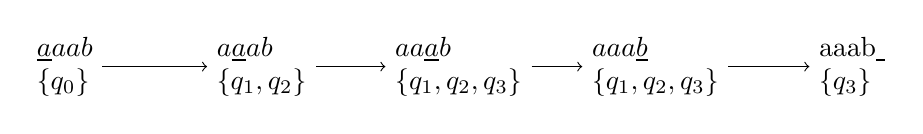
\begin{tikzpicture}[node distance=2.5cm,auto]     \node (one) [align=left] {$\underline{a}aab$\\$\left\{ q_{0}\right\} $};     \node (two) [right of=one,align=left] {$a\underline{a}ab$\\$\left\{ q_{1}, q_{2} \right\} $};     \node (three) [right of=two,align=left] {$aa\underline{a}b$\\$\left\{ q_{1}, q_{2}, q_{3} \right\} $};     \node (four) [right of=three,align=left] {$aaa\underline{b}$\\$\left\{ q_{1}, q_{2}, q_{3} \right\} $};     \node (five) [right of=four,align=left] {aaab\underline{ }\\$\left\{q_{3} \right\} $};     \path[->] (one) edge node {} (two);     \path[->] (two) edge node {} (three);     \path[->] (three) edge node {} (four);     \path[->] (four) edge node {} (five); \end{tikzpicture}

\label{thompson-exec}}\caption{Example of the Thompson algorithm.}
\end{figure}

\begin{example}
The automaton $A$ of Figure \ref{thompson-aut} matches the string
$\mathbf{s}=$'aaab'. Figure \ref{thompson-exec} illustrates the
execution of $A$ on $\mathbf{s}$. Notice how runs that end up in
the same state are naturally merged. For instance, if we are in $q_{1}$
and we read an $a$ we can go to $q_{3}$, but we can also read an
$a$ while in $q_{3}$, remaining in that state. Nonetheless, in the
cases where both $q_{1}$ and $q_{3}$ are in the current state set,
$q_{3}$ appears only once in the next. This is because the two originally
distinct runs are now equivalent. This lets the algorithm keep a reduced
list of current states, and justifies the runtime complexity presented.
\end{example}

One interesting implementation of the Thompson algorithm views an
NFA as a program that can be executed by a virtual machine on a string.
This method is described in \cite{cox_regular_2009}. 

\subsubsection{The Virtual Machine Implementation}

In this implementation, a NFA (or a regex) is converted into a program,
written in a simple assembly language with few instructions. The basic
instructions are character match (CHAR), string match (MATCH), and
control flow instructions (SPLIT and JUMP). A virtual machine is provided,
which treats each concurrent run on a string $\mathbf{s}$ as a conceptual
thread. The virtual machine advances all the threads in lockstep,
in the spirit of the Thompson approach. Actual implementations can
enforce a policy for ambiguous matches. Different threads that reach
the same instruction in a program are merged. 

The main advantage of this method is that it is easy to enrich the
assembly language with new instructions, in order to support new features.
To execute new instructions, modyifing the virtual machine is required.
For instance, capturing groups can be implemented by equipping each
thread with an array of saved pointers that are grouped by two: the
first element would point to the beginning of a span of text and the
second one would point to its end. Then, a SAVE instruction could
be added, that would make the virtual machine record the current position
in the input into the pointer specified by the instruction.

\begin{figure}
\centering

\subfloat[A program for the regex $a^{+}b^{\ast}$.]{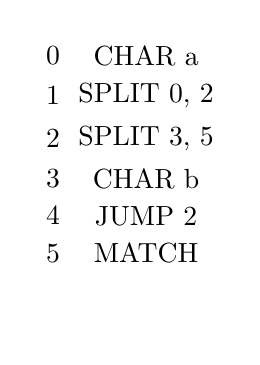
\begin{tikzpicture} \matrix [ampersand replacement=\&]{ 	\node {0}; \& \node {CHAR a};    \\ 	\node {1}; \& \node {SPLIT 0, 2};\\ 	\node {2}; \& \node {SPLIT 3, 5};\\ 	\node {3}; \& \node {CHAR b};    \\ 	\node {4}; \& \node {JUMP 2};    \\ 	\node {5}; \& \node {MATCH};     \\ 	\node {}; \& \node {};     \\ 	\node {}; \& \node {};     \\ 	\node {}; \& \node {};     \\
}; \end{tikzpicture}

\label{prog}}\subfloat[A program for the regex $\left(a^{+}\right)\left(b^{\ast}\right)$.]{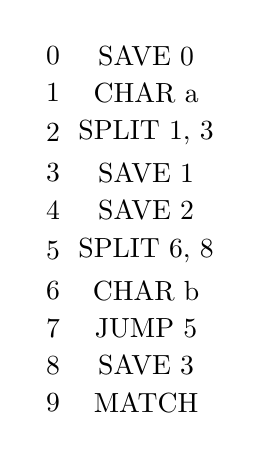
\begin{tikzpicture} \matrix [ampersand replacement=\&]{ 
	\node{0}; \& \node {SAVE 0};    \\ 	\node{1}; \& \node {CHAR a};    \\ 	\node{2}; \& \node {SPLIT 1, 3};\\ 	\node{3}; \& \node {SAVE 1};    \\ 	\node{4}; \& \node {SAVE 2};    \\ 	\node{5}; \& \node {SPLIT 6, 8};\\ 	\node{6}; \& \node {CHAR b};    \\ 	\node{7}; \& \node {JUMP 5};    \\ 	\node{8}; \& \node {SAVE 3};    \\ 	\node{9}; \& \node {MATCH};     \\
}; \end{tikzpicture}

\label{prog-capt}}\caption{Example programs.}

\end{figure}

\begin{example}
The program shown in Figure \ref{prog} can be used to match the regular
expression $a^{+}b^{*}$. SPLIT instructions explictly divide a thread
into two, telling each of the generated threads which position in
the program to reach. The program in Figure \ref{prog-capt} matches
the same expression as the one in Figure \ref{prog}, but it retains
the substrings matching the subexpressions between parentheses too.

\begin{figure}
\centering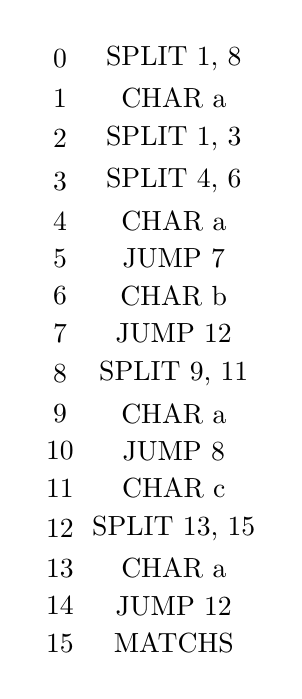
\begin{tikzpicture} \matrix [ampersand replacement=\&]{ 
	\node{0}; \& \node {SPLIT 1, 8};    \\ 	\node{1}; \& \node {CHAR a};    \\ 	\node{2}; \& \node {SPLIT 1, 3};\\ 	\node{3}; \& \node {SPLIT 4, 6};    \\ 	\node{4}; \& \node {CHAR a};    \\ 	\node{5}; \& \node {JUMP 7};\\ 	\node{6}; \& \node {CHAR b};    \\ 	\node{7}; \& \node {JUMP 12};    \\ 	\node{8}; \& \node {SPLIT 9, 11};    \\ 	\node{9}; \& \node {CHAR a};     \\ 	\node{10}; \& \node {JUMP 8};     \\ 	\node{11}; \& \node {CHAR c};     \\ 	\node{12}; \& \node {SPLIT 13, 15};     \\ 	\node{13}; \& \node {CHAR a};     \\ 	\node{14}; \& \node {JUMP 12};     \\ 	\node{15}; \& \node {MATCHS};     \\
}; \end{tikzpicture}

\label{prog-aut}\caption{A program for the automaton $A$ of Figure \ref{thompson-aut}.}
\end{figure}
\end{example}

\begin{example}
The program shown in Figure \ref{prog-aut} corresponds to the automaton
$A$ of Figure \ref{thompson-aut}. Notice how the $\varepsilon$-transition
between $q_{0}$ and $q_{2}$ is automatically omitted from the program.
Blocks of SPLIT instructions correspond to multiple outgoing transitions
from a state. JUMP instructions are used to merge execution branches. 
\end{example}


\subsection{Ordered Binary Decision Diagrams}

Ordered Binary Decision Diagrams (OBDDs) are tree-like structures,
that can be used to efficiently represent, manipulate and evaluate
boolean formulas. One of their advantages is that first order logic
quantifiers can be easily supported by performing a series of operations
that change the structure of an OBDD opportunely. In \cite{Yang:2012:FSE:2396556.2396594},
it is shown how to encode NFAs as OBDDs, with support for submatch
extraction. Then, a procedure for evaluating a string by using an
OBDD representation of a NFA is described.

Given a regular expression $r$ of size $m$ and a string of size
$n$, the runtime cost of this approach is shown to be between $O\left(m\right)$
and $O\left(mn\right)$. The authors of \cite{Yang:2012:FSE:2396556.2396594}
suggest that this approach performs best when matching patterns are
combined togheter.

\subsection{Kleenex}

A \emph{transducer} is a kind of finite state machine whose main difference
with an NFA is that it has an \emph{output tape}. Thus, the transition
function of a transducer is enriched with \emph{output actions.} Output
actions can be used to write to the output tape, thus providing a
way to support submatch extraction.

In \cite{Grathwohl:2016:KCN:2914770.2837647}, the Kleenex language
is presented. It can be used to specify context free grammars, representing
regular expressions with capturing groups. A Kleenex program is converted
to a transducer, which is in turn decomposed into an \emph{oracle
machine} and an \emph{action machine}. The oracle machine traverses
an input string trying to match it (according to a disambiguation
policy), while the action machine performs the ouput actions. 

\section{Implementation}

In the system, core spanners are represented by well-behaved eVset-automata,
for which a set of string equality constraints can be specified on
pairs of their span variables. Moreover, the implementation fixes
$\textrm{SVars}=\mathbb{N}$. Hence, span variables are identified
by nonnegative integers. The system can be used in two modes: 
\begin{description}
\item [{compilation}] reads an AQL core fragment specification and produces
an equivalent core spanner representation;
\item [{evaluation}] evaluates a core spanner representation on a series
of text documents, returning, for each of them, a $\left(V,\mathbf{s}\right)$-relation
as output.
\end{description}

\subsection{Compilation Mode}

The compilation mode allows to easily compose spanner representations
to obtain more complex ones. The composition process is performed
according to an input AQL core fragment, written in an ad-hoc syntax
that linearizes its operator tree. \emph{// I will put an example. }

The compilation mode supports all the operators described in Section
\ref{subsec:Algebras-of-Spanners}. For projection, union and natural
join, the constructions described in Theorems \ref{ext-proj}, \ref{ext-union}
and \ref{ext-join} are respectively used (keep in mind that core
spanners are represented by well-behaved eVset-automata). String equality
selection operations are simply reported in the resulting representation,
for use of the evaluation engine. \emph{// Need to describe the 'isFollowedBy'
join here.}

\subsection{Evaluation Mode}

\begin{algorithm}
$E\longleftarrow\left\{ \textrm{core spanner representation}\right\} $

for document in inputDirectory do

begin
\begin{enumerate}
\item $\left\{ \textrm{Read document into main memory}\right\} $
\item $R\longleftarrow E\left(\textrm{document}\right)$
\item $\left\{ \textrm{Write \ensuremath{R} to disk}\right\} $
\end{enumerate}
\caption{\label{alg:The-execution-algorithm}The execution algorithm of a core
spanner representation on a set of input documents.}

\end{algorithm}

The evaluation mode requires as input a core spanner representation
and the path of the directory containing the text documents to span.
The execution algorithm, represented by Algorithm \ref{alg:The-execution-algorithm},
is similar to that of SystemT, whose high-level structure is described
by Algorithm \ref{alg:Annotating-all-local}. In particular, Algorithm
\ref{alg:The-execution-algorithm} conforms to document-at-a-time
processing as well. On the other hand, the results are written to
a separate file, instead of annotating the input documents, as in
Algorithm \ref{alg:Annotating-all-local}.

\medskip{}

The engine that evaluates a spanner representation on a document draws
inspiration from the Thompson approach, described in Subsection \ref{subsec:The-Thompson-Approach}.
The procedure defined by this approach can't be used as is. This is
because when evaluating an eVset-automaton $A$ on a string $\textrm{\ensuremath{\mathbf{s}}}$,
we are interested in all the $\mathbf{s}$-tuples defined by the runs
belonging to $\textrm{ARuns}\left(A,\mathbf{s}\right)$, instead of
a single match. Subsequently, the implementation of the engine doesn't
discard any of the feasible runs in $\textrm{ARuns}\left(A,\mathbf{s}\right)$.

Initially, the implementation followed the Virtual Machine method:
a core spanner representation was converted into an NFA program and
executed by a modified implementation of the virtual machine. However
this implementation revealed itself to be slow. Thus, the engine was
changed so that it directly uses input eVset-automata: in this implementation,
a set of current runs is maintained, and each run is advanced by following
the outgoing transitions of its current state. All the runs are advanced
in lockstep. There's another difference with the original Thompson
approach: operation transitions, which may be considered as a special
kind of $\epsilon$-transitions, aren't followed iteratively, thus
different runs may point to different positions of the input string
at the same moment.

\chapter{Experiments}

After the development of the system, an experimental validation phase
followed. The experiments were designed to test whether the evaluation
approach described in this paper (converting a query into a well-behaved
eVset-automaton and using a modified regular expression engine to
find matches) brings performance benefits over the approach of SystemT.
In order to make a fair comparison, a subsystem that imitates SystemT
was developed. This systems doesn't support the optimization techniques
described in \cite{4497502,Krishnamurthy:2009:SSD:1519103.1519105}.

\section{A Subsystem for the Algebraic Approach}

The subsystem implements the operators of the algebra as operations
on $\left(V,\mathbf{s}\right)$-relations, that return a new $\left(V,\mathbf{s}\right)$-relation.
\emph{// To be continued...}

\section{Queries}

\emph{// Description of the benchmark queries will go here...}

\section{Experimental Results}

\emph{// Just the diagrams for now. Discussion will go here.}

\begin{figure}
\pgfplotstableread[row sep=\\,col sep=&]{     interval      & baseT \\     Action        & 13.03 \\     Aspect        & 16.75 \\     Attribute     & 18.67 \\     Genre         & 20.23 \\     MovieKeyword  & 13.30 \\     Name          & 12.38 \\     PlotClue      & 16.83 \\     Role          & 14.32 \\     RoleClue 	  & 12.25 \\     Sentiment     & 15.45 \\     Title         & 12.03 \\     }\mydata
\begin{tikzpicture}     \begin{axis}[             ybar,             bar width=.5cm,             width=\textwidth,             height=.5\textwidth,             symbolic x coords={Action,Aspect,Attribute,Genre,MovieKeyword,Name,PlotClue,Role,RoleClue,Sentiment,Title},             xtick=data, 	    xticklabel style={ 		inner sep=0pt, 		anchor=north east, 		rotate=45 	    },             nodes near coords,             nodes near coords align={vertical},             ymin=0,ymax=25,             ylabel={Running Time (min.)},         ]         \addplot table[x=interval,y=baseT]{\mydata};     \end{axis} \end{tikzpicture}

\caption{}
\end{figure}
\begin{figure}
\centering

\pgfplotstableread[row sep=\\,col sep=&]{     interval & cls & vst \\     Query 1     & 22.93  & 13.23 \\     Query 2     & 29.33 & 18.25 \\     Query 3   & 26.95 & 13.77 \\     }\mydata
\begin{tikzpicture}     \begin{axis}[             ybar,             bar width=.5cm,             width=.6\textwidth,             height=.5\textwidth,             symbolic x coords={Query 1,Query 2,Query 3},             xtick=data, 	    xticklabel style={ 		inner sep=0pt, 		anchor=north east, 		rotate=45 	    },             nodes near coords,             nodes near coords align={vertical},             ymin=0,ymax=35,             ylabel={Running Time (min.)},         ]         \addplot table[x=interval,y=cls]{\mydata}; 	\addplot table[x=interval,y=vst]{\mydata};     \end{axis} \end{tikzpicture}

\caption{}

\end{figure}
\begin{figure}
\pgfplotstableread[row sep=\\,col sep=&]{     interval  & cls   & vst   & vstF  \\     Query 4   & 108.02 & 88.63 & 0 \\     Query 5   & 134.33 & 97.87 & 86.17 \\     Query 6   & 136.38 & 135.17 & 100.98 \\     Query 7   & 117.67 & 381.02 & 188.15 \\     }\mydata
\begin{tikzpicture}     \begin{axis}[             ybar,             bar width=.5cm,             width=\textwidth,             height=.5\textwidth,             symbolic x coords={Query 4,Query 5,Query 6,Query 7},             xtick=data, 	    xticklabel style={ 		inner sep=0pt, 		anchor=north east, 		rotate=45 	    },             nodes near coords,             nodes near coords align={vertical},             ymin=0,ymax=400,             ylabel={Running Time (min.)},         ]         \addplot table[x=interval,y=cls]{\mydata}; 	\addplot table[x=interval,y=vst]{\mydata}; 	\addplot table[x=interval,y=vstF]{\mydata};     \end{axis} \end{tikzpicture}

\caption{}

\end{figure}
\begin{figure}
\pgfplotstableread[row sep=\\,col sep=&]{     interval  & cls   & vst  \\     Query 8   & 38.52 & 14.08 \\     Query 9   & 34.55 & 14.10 \\     Query 10  & 50.08 & 16.6 \\     }\mydata
\begin{tikzpicture}     \begin{axis}[             ybar,             bar width=.5cm,             width=\textwidth,             height=.5\textwidth,             symbolic x coords={Query 8,Query 9,Query 10},             xtick=data, 	    xticklabel style={ 		inner sep=0pt, 		anchor=north east, 		rotate=45 	    },             nodes near coords,             nodes near coords align={vertical},             ymin=0,ymax=60,             ylabel={Running Time (min.)},         ]         \addplot table[x=interval,y=cls]{\mydata}; 	\addplot table[x=interval,y=vst]{\mydata};     \end{axis} \end{tikzpicture}

\caption{}

\end{figure}
\begin{figure}
\pgfplotstableread[row sep=\\,col sep=&]{     interval  & cls   & vst  \\     Query 11  & 82.63 & 30.98 \\     Query 12  & 117.57 & 47.72 \\     Query 13  & 132.18 & 61.7 \\     Query 14  & 133.63 & 79.05 \\     }\mydata
\begin{tikzpicture}     \begin{axis}[             ybar,             bar width=.5cm,             width=\textwidth,             height=.5\textwidth,             symbolic x coords={Query 11,Query 12,Query 13,Query 14},             xtick=data, 	    xticklabel style={ 		inner sep=0pt, 		anchor=north east, 		rotate=45 	    },             nodes near coords,             nodes near coords align={vertical},             ymin=0,ymax=200,             ylabel={Running Time (min.)},         ]         \addplot table[x=interval,y=cls]{\mydata}; 	\addplot table[x=interval,y=vst]{\mydata};     \end{axis} \end{tikzpicture}

\caption{}

\end{figure}

\selectlanguage{english}%

\chapter{Conclusions}

\section{Discussion}

blabla

\section{Future Works}

blabla

\section{Promising Directions}

blabla

\selectlanguage{american}%




\selectlanguage{english}%
\bibliographystyle{apalike}
\nocite{*}
\bibliography{survey,systemT1,systemT2,spanners,datalog,regex,vm,regex2,obdd,kleenex}

\selectlanguage{american}%

\appendix

\chapter{Do we need an Appendix?}

\selectlanguage{english}%
maybe...

\selectlanguage{american}%



\printindex{} 
\end{document}
